\documentclass[a4paper,12pt,oneside]{scrbook}
\KOMAoptions{
    chapterprefix=true,
    parskip=half,
    captions=tableheading,
    draft=false
}

\usepackage{iftex}

% Activar números de línea
% \usepackage{lineno}
% \linenumbers
% \setlength\linenumbersep{5pt}
% \renewcommand\linenumberfont{\normalfont\tiny\sffamily\color{gray}}

\usepackage[spanish,es-nolists,es-tabla,es-noindentfirst]{babel}
\usepackage[hidelinks]{hyperref}

\renewcommand{\listtablename}{Índice de tablas}    
\renewcommand{\listfigurename}{Índice de figuras}
\newcommand*{\listofloaname}{Índice de algoritmos}

\addto\extrasspanish{
    \renewcommand{\sectionautorefname}{Apartado}
    \renewcommand{\subsectionautorefname}{Apartado}
    \renewcommand{\subsubsectionautorefname}{Apartado}
}

% Márgenes del documento
\usepackage{geometry}
\geometry{left=2cm, right=2cm, top=2cm, bottom=3.3cm}

% Interlineado 1.5
% \onehalfspacing

% Sangría 
% Ojo, la guía de KOMA-Script sugiere usar espaciado o sangría para delimitar los párrafos,
% pero no ambas cosas porque es redundante. Descomentando la siguiente línea se activa la sangría.
% \setlength{\parindent}{0.5cm}

% Configuración de fuentes
\ifPDFTeX
    \usepackage[T1]{fontenc}
    \usepackage[utf8]{inputenc}
    \usepackage{lmodern}
    \usepackage{amsmath}
    \usepackage{amssymb}
    \usepackage{textcomp}
    \usepackage[scale=0.85]{sourcecodepro}

    \renewcommand{\familydefault}{\sfdefault}
    \newcommand{\lmromanfont}{\rmfamily}
\else % XeLaTeX / LuaLaTeX
    \usepackage{fontspec}
    \usepackage{amsmath}
    \usepackage{unicode-math}   % Incluye Latin Modern Math
    
    \setmainfont{Latin Modern Sans}[
        Ligatures=TeX,
        % Necesario porque Latin Modern Sans no incluye estilo small caps
        SmallCapsFont=Latin Modern Roman Caps
    ]
    \setsansfont{Latin Modern Sans}[Ligatures=TeX]
    \setmonofont{Source Code Pro}[Scale=MatchLowercase]
    % \setmonofont[Scale=MatchLowercase]{Fira Mono}
    \newfontfamily{\lmromanfont}{Latin Modern Roman}
\fi

% Configuración de listas no numeradas
\setkomafont{itemizelabel}{\lmromanfont}
\renewcommand{\labelitemii}{$\circ$}
\renewcommand{\labelitemiii}{$\diamond$}
\renewcommand{\labelitemiv}{$\triangleright$}

% Citas
\usepackage{csquotes}
\renewcommand{\mkbegdispquote}[2]{«}
\renewcommand{\mkenddispquote}[2]{#1»#2}

%% Bibliografía
% Numérica (ordenada por orden de aparación)
\usepackage[style=numeric-comp,sorting=none,backend=biber]{biblatex}
\defbibnote{note}{Las siguientes referencias bibliográficas se presentan en orden de aparición en el texto.\par\bigskip}
% APA (ordenada por autor, año y título)
% \usepackage[style=apa,sorting=nyt,backend=biber]{biblatex}
% \defbibnote{note}{Las siguientes referencias bibliográficas se presentan en orden alfabético por autor. Las referencias con más de un autor aparecen ordenadas en base al primero de los mismos.\par\bigskip}

\addbibresource{referencias.bib}

\usepackage{caption}
\usepackage{enumitem}
\usepackage{float}
\usepackage{graphicx}
\usepackage{lipsum}
\usepackage{microtype}
\usepackage{pdflscape}
\usepackage{rotating}
\usepackage{subcaption}
\usepackage[table]{xcolor}

\usepackage{siunitx}
\ifPDFTeX
    \newcommand{\perthousand}{\textperthousand}
\else
    % XeLaTeX / LuaLaTeX
    \newcommand{\perthousand}{‰}
\fi

% Tablas
\usepackage{array} 
\usepackage{booktabs}
\usepackage{longtable}
\usepackage{multirow}
\usepackage{tabularx}
% Definir columnas para alineación a la derecha o centro y ajuste automático
\newcolumntype{R}{>{\raggedleft\arraybackslash}X}
\newcolumntype{C}{>{\centering\arraybackslash}X}
% Definir tipos de columnas en modo matemático
% Ver pag. 3 en la documentación del paquete array:
\newcolumntype{M}{>{$}c<{$}}
\newcolumntype{L}{>{$}l<{$}}
\newcolumntype{N}{>{$}r<{$}}
% Distancia entre filas
\renewcommand*{\arraystretch}{1.5}

% Código con coloreado de sintaxis
\usepackage{scrhack}            % Para evitar un warning sobre \float@addtolist
\usepackage{listings}
\renewcommand{\lstlistingname}{Listado}
\input{settings/listings}       % Estilo y definiciones para lenguajes adicionales

% Descripción de algoritmos en pseudocódigo
\usepackage[chapter]{algorithm}
\usepackage{algpseudocodex}
\floatname{algorithm}{Algoritmo}
\captionsetup[algorithm]{labelfont=bf, labelsep=default}

\newenvironment{abstract}[1][\abstractname]{
    \cleardoublepageusingstyle{empty}
    \thispagestyle{empty}
    \begin{center}\textbf{#1}\end{center}
    \begin{itshape}\par\noindent%
}
{\end{itshape}}

\newenvironment{keywords}[1][Keywords]
{\vspace{7pt}\par\noindent\textup{\textbf{#1: }}\begin{upshape}}
{\end{upshape}}

\newcommand{\license}[2]{%
\begin{center}
    \begin{minipage}{0.8\textwidth}   
        \begin{center}
            \includegraphics[width=4.66cm]{#1}\\[12pt]
            {\Large #2}
        \end{center}
    \end{minipage}
\end{center}
}

% Formato de capítulos
% Eliminar el punto y reducir el espacio entre el prefijo y el nombre del capítulo 
\renewcommand*{\chapterformat}{%
    \mbox{\chapappifchapterprefix{\nobreakspace}\thechapter
    \IfUsePrefixLine{}{\enskip}}}
\renewcommand{\chapterheadmidvskip}{\vskip 0pt}

% Formato de los títulos en figuras y tablas
\renewcommand*{\figureformat}{\figurename~\thefigure}
\renewcommand*{\tableformat}{\tablename~\thetable}

% Redefinición de las entradas de los capítulos en la tabla de contenidos
% para que aparezca el prefijo.
\let\originaladdchaptertocentry\addchaptertocentry
\renewcommand*{\addchaptertocentry}[2]{%
  \IfArgIsEmpty{#1}{% Entrada sin número
    \originaladdchaptertocentry{#1}{#2}%
  }{% Entrada con número
    % Eliminar el número y poner el prefijo directamente en el título del capítulo
    \originaladdchaptertocentry{}{\chapapp~#1\autodot\space#2}%
  }%
}

\begin{document}   

%%%%%%%%%%%%%%%%%%%%%%%%%%%%%%%%%%%%%%%%%%%%%%%%%%%%%%%%%%%%%%%%%%%%%%%%%%%%%%%
% Portada y metadatos
%%%%%%%%%%%%%%%%%%%%%%%%%%%%%%%%%%%%%%%%%%%%%%%%%%%%%%%%%%%%%%%%%%%%%%%%%%%%%%%

% Metadatos del PDF
\hypersetup{
    pdftitle='Título del trabajo',
    pdfauthor='Nombre y Apellidos',
    pdfsubject={Trabajo de Fin de Grado},
}

\pagestyle{empty}
\newcommand{\HRule}{\rule{\linewidth}{0.3mm}}
{
    \setlength{\parindent}{0mm}
    \setlength{\parskip}{0mm}
    
    \vspace*{1.20cm}
    
\includegraphics[width=9.81cm]{images/logos/escuela-ingenieria-tecnologia-original}
    \vspace*{\stretch{0.9}}
    
    {\centering
    \fontsize{32pt}{32pt}\selectfont Trabajo de Fin de Grado\\[10pt]
    \fontsize{20pt}{20pt}\selectfont Grado en Ingeniería Informática\par}
    \HRule\vspace*{-2mm}
    \begin{flushright}
        {\fontsize{32pt}{32pt}\selectfont Marketplace colaborativo de aparcamiento Peer-to-Peer\par
        \vspace*{3mm}
        \fontsize{18pt}{18pt}\selectfont \textit{Peer-to-Peer Collaborative Parking Marketplace}\par
        \vspace*{11mm}
        \fontsize{16pt}{16pt}\selectfont Hugo González Pérez
        }\vspace*{12mm}
    \end{flushright}
    \HRule
    
    \vspace*{\stretch{1}}
    \begin{center}
        \fontsize{18pt}{18pt}\selectfont La Laguna, \today
    \end{center}
}

%%%%%%%%%%%%%%%%%%%%%%%%%%%%%%%%%%%%%%%%%%%%%%%%%%%%%%%%%%
% Certificado
%%%%%%%%%%%%%%%%%%%%%%%%%%%%%%%%%%%%%%%%%%%%%%%%%%%%%%%%%%
\frontmatter
\cleardoublepageusingstyle{empty}
\thispagestyle{empty}

{
\setlength\parindent{0pt}
    D. \textbf{Francisco Javier Rodríguez González}, con N.I.F. 43.618.712-V profesor Asociado de Universidad adscrito al Departamento de Ingeniería Informática y de Sistemas de la Universidad de La Laguna, como tutor
    
    \bigskip
    D. \textbf{Alejandro Pérez Nava}, con N.I.F. 43.821.179-S profesor Asociado de Universidad adscrito al Departamento de Ingeniería Informática y de Sistemas de la Universidad de La Laguna, como cotutor
    
    \bigskip
    \bigskip
    \textbf{C E R T I F I C A (N)}

    \bigskip
    Que la presente memoria titulada:
    
    \bigskip
    \begin{quote}
    \textit{``Marketplace colaborativo de aparcamiento Peer-to-Peer''}
    \end{quote}
    
    \bigskip
    \noindent ha sido realizada bajo su dirección por D. \textbf{Hugo González Pérez}, con N.I.F 78.824.986-F.
    
    \bigskip
    Y para que así conste, en cumplimiento de la legislación vigente y a los efectos
    oportunos, firman la presente en La Laguna a \today
}

%%%%%%%%%%%%%%%%%%%%%%%%%%%%%%%%%%%%%%%%%%%%%%%%%%%%%%%%%%
% Agradecimientos
%%%%%%%%%%%%%%%%%%%%%%%%%%%%%%%%%%%%%%%%%%%%%%%%%%%%%%%%%%
\cleardoublepageusingstyle{empty}
\thispagestyle{empty}

\begin{flushright}
    \setlength{\parindent}{0mm}
    {\huge Agradecimientos}
    \vspace{15mm}
    
    \begin{large}
        \begin{minipage}{1\textwidth} 
            A mi familia, especialmente a mis padres, por su apoyo incondicional y por creer siempre en mí, dándome la fuerza necesaria para superar cada etapa de mi formación académica. Sin su sacrificio y cariño, nada de esto habría sido posible. A mis amigos y compañeros, por los momentos compartidos, las largas jornadas de estudio y por hacer que este camino fuera mucho más ameno. Por último, a la Universidad de La Laguna por brindarme el entorno y las herramientas necesarias para formarme como profesional.
        \end{minipage}
    \end{large}
\end{flushright}

%%%%%%%%%%%%%%%%%%%%%%%%%%%%%%%%%%%%%%%%%%%%%%%%%%%%%%%%%%
% Licencia
%%%%%%%%%%%%%%%%%%%%%%%%%%%%%%%%%%%%%%%%%%%%%%%%%%%%%%%%%%
\cleardoublepageusingstyle{empty}
\thispagestyle{empty}

{\noindent\LARGE Licencia}
\vspace{15mm}

\license{images/licenses/by-nc-nd.eu}{© Esta obra está bajo una licencia de Creative Commons Reconocimiento-NoComercial-SinObraDerivada 4.0 Internacional.}

\bigskip

%%%%%%%%%%%%%%%%%%%%%%%%%%%%%%%%%%%%%%%%%%%%%%%%%%%%%%%%%%
% Resumen
%%%%%%%%%%%%%%%%%%%%%%%%%%%%%%%%%%%%%%%%%%%%%%%%%%%%%%%%%%
\begin{abstract}
El objetivo de este trabajo ha sido... bla, bla, bla, bla, bla, bla, bla, bla, bla...

La competencia [E6], que figura en la guía docente, indica que en la memoria del trabajo se ha de incluir: antecedentes, problemática o estado del arte, objetivos, fases y desarrollo del proyecto, conclusiones, y líneas futuras.

Se ha incluido el apartado de 'Licencia' con todas las posibles licencias abiertas (Creative Commons). En el caso en que se decida hacer público el contenido de la memoria, habrá que elegir una de ellas (y borrar las demás). La decisión de hacer pública o no la memoria se indica en el momento de subir la memoria a la Sede Electrónica de la ULL, paso necesario en el proceso de presentación del TFG.

El documento de memoria debe tener un máximo de 50 páginas.

No se deben dejar páginas en blanco al comenzar un capítulo, ya que el documento no está pensado para ser impreso sino visionado con un lector de PDF.

También es recomendable usar márgenes pequeños, ya que, al firmar digitalmente por la Sede Electrónica, se coloca un marco alrededor del texto original.

El tipo de letra base ha de ser de 12 pt.

\begin{keywords}[Palabras clave]
Palabra reservada1, Palabra reservada2,...
\end{keywords}
\end{abstract}

%%%%%%%%%%%%%%%%%%%%%%%%%%%%%%%%%%%%%%%%%%%%%%%%%%%%%%%%%
\cleardoublepageusingstyle{empty}
\thispagestyle{empty}

\begin{abstract}[Abstract]
Here should be the abstract in a foreing language...

\begin {keywords}
Keyword1, Keyword2, Keyword3,...
\end{keywords}
\end{abstract}

%%%%%%%%%%%%%%%%%%%%%%%%%%%%%%%%%%%%%%%%%%%%%%%%%%%%%%%%%
\pagestyle{plain}
\cleardoublepage
\setcounter{page}{1} 

\tableofcontents
\listoffigures
\listoftables
%\listofalgorithms

%%%%%%%%%%%%%%%%%%%%%%%%%%%%%%%%%%%%%%%%%%%%%%%%%%%%%%%%%%
% Contenidos
%%%%%%%%%%%%%%%%%%%%%%%%%%%%%%%%%%%%%%%%%%%%%%%%%%%%%%%%%%
\mainmatter

\chapter{Introducción}
\label{ch:introducción}
\section{Definición del problema}

No es una novedad que el crecimiento del \textit{parque móvil}\footnote{\textbf{Parque móvil}: Conjunto total de vehículos registrados y en circulación en una determinada región o país.} y el auge del turismo en las Islas Canarias y sobre todo en Tenerife han provocado que encontrar aparcamiento en prácticamente cualquier lugar resulte cada vez más difícil. En las zonas de alta densidad, como puede ser el \textbf{área metropolitana}, el problema es aún más acentuado, donde tanto residentes como visitantes diariamente sufren un desequilibrio crítico entre oferta y demanda de espacio urbano.

En muchas vías de Tenerife, este problema se manifiesta de forma recurrente en los principales ejes urbanos. Cualquier conductor que transite por la zona que hay entre Santa Cruz de Tenerife y San Cristóbal de La Laguna puede verse atrapado en atascos que, en trayectos de apenas diez kilómetros, generan pérdidas de tiempo significativas y degradan la calidad de vida. Sin embargo, el problema no reside únicamente en la congestión de vías principales como la \textit{(TF-5)}\footnote{\textbf{TF-5}: Es la principal autopista del norte de Tenerife, que conecta Santa Cruz de Tenerife con el área metropolitana y los municipios del norte de la isla.}, sino en la dificultad añadida de encontrar un hueco libre al llegar al destino. De hecho, se estima que hasta un 35\% del tráfico urbano en horas punta está compuesto por vehículos que circulan en bucle buscando estacionamiento~\cite{elpais2025trafico35}, lo que contribuye innecesariamente a la contaminación acústica y a las emisiones de gases de efecto invernadero \textit{(GEI)}\footnote{\textbf{GEI}: Los gases de efecto invernadero son aquellos que contribuyen al calentamiento global al retener el calor en la atmósfera, como el dióxido de carbono (CO$_2$).}.

Moverse por Santa Cruz de Tenerife en hora punta se ha convertido en una prueba de paciencia: el \textit{TomTom Traffic Index}~\cite{tomtom2026} registró en 2025 que los conductores perdieron una media de 52 horas atrapados en el tráfico y un índice de congestión del 34,8\%, lo que equivale a pasar más de dos días enteros al año prácticamente parados en cola. El gran embudo diario llega con  el atardecer, cuando la velocidad cae a unos desesperantes 28 km/h y la congestión alcanza el 55,7\%.

Resulta irónico que, mientras cientos de conductores pierden tiempo y combustible buscando aparcamiento, estas plazas permanezcan vacías durante gran parte del día o incluso durante periodos vacacionales. Este desaprovechamiento de un recurso escaso pone de manifiesto una clara ineficiencia en la gestión del espacio disponible.

Es por ello que, a partir de este gran contraste, nace la motivación de \textbf{Parky} y su principal objetivo: explorar cómo se puede conectar a los propietarios de estas plazas privadas poco usadas con conductores que requieren estacionar su vehículo, facilitando por medio de tecnologías digitales una gestión más inteligente y eficiente de los recursos urbanos existentes.

\medskip
\noindent\textit{Nota terminológica:} a lo largo de la memoria, los términos \textit{arrendador} y \textit{propietario de plaza} se emplean de forma equivalente para referirse al titular del garaje que lo pone en alquiler; del mismo modo, \textit{arrendatario} y \textit{conductor} designan indistintamente a quien realiza la reserva.

\section{Justificación}
\label{sec:justificación}

Parky busca responder a tres factores que convergen en el contexto urbano de 2026: presión normativa, eficiencia económica y madurez tecnológica.

En primer lugar, desde la perspectiva de la \textbf{sostenibilidad y presión regulatoria}, el proyecto responde a la obligatoriedad de implementar Zonas de Bajas Emisiones \textit{(ZBE)} en municipios de más de 50.000 habitantes, como es el caso de Santa Cruz de Tenerife y San Cristóbal de La Laguna. Una parte sustancial del tráfico urbano es generado exclusivamente por la búsqueda de estacionamiento. Facilitar una plataforma \textit{(P2P)}\footnote{\textbf{P2P}: Sistema digital que permite a personas o empresas realizar transacciones directas entre sí, sin la necesidad de intermediarios tradicionales como bancos o grandes empresas.} permite una transición hacia una movilidad más ordenada, reduciendo significativamente las emisiones de gases y el ruido en el centro de las ciudades, alineándose así con los objetivos de las denominadas \textit{Smart Cities}\footnote{\textbf{Smart Cities}: es un entorno urbano que utiliza tecnologías avanzadas, como el Internet de las Cosas (IoT), la inteligencia artificial (IA), el big data y las TIC (Tecnologías de la Información y Comunicación), para mejorar la calidad de vida de sus habitantes, optimizar la gestión de recursos y promover el desarrollo sostenible.}.

En segundo lugar, la \textbf{eficiencia social y económica} del modelo P2P está respaldada por datos: la movilidad compartida registra una tasa de crecimiento anual compuesta (CAGR)\footnote{\textbf{CAGR} (\textit{Compound Annual Growth Rate}): indicador financiero que mide la tasa de crecimiento anual compuesta de una inversión o mercado durante un período determinado, asumiendo la reinversión de los beneficios.} del 14,8\% hasta 2030~\cite{grandviewresearch2022}. \textbf{Parky} permite a los propietarios obtener entre 150 € y 300 € mensuales por una plaza infrautilizada, mientras que ofrece al conductor un ahorro directo de tiempo ya que se dedica de media 24 horas anuales solo a buscar hueco~\cite{inrix2022}.

Por último, la \textbf{viabilidad tecnológica} está respaldada por la madurez del ecosistema disponible. Las APIs de geolocalización, las pasarelas de pago P2P y las bases de datos con seguridad a nivel de fila existen, están documentadas y tienen precios accesibles para un prototipo. El mismo conductor que hoy circula en bucle puede reservar y acceder a una plaza privada en menos de dos minutos desde el móvil.

\section{Estado del arte}
\label{sec:estado-del-arte}

Las plataformas de aparcamiento en 2026 se organizan en cuatro categorías con modelos de negocio y barreras de entrada distintas que se describen a continuación.

\subsection{Aplicaciones de zona regulada}

Las plataformas de zona regulada digitalizan el cobro de tasas de estacionamiento en vía pública mediante contratos con los ayuntamientos. Sin ese convenio, no pueden operar en ninguna ciudad. Esta dependencia institucional define su modelo de expansión y limita su presencia a los municipios que han licitado el servicio.

\textbf{EasyPark}~\cite{easypark2024} opera en más de 4.200 ciudades de 21 países, con más de 6.000 operadores de aparcamiento integrados, resultado de una estrategia de adquisiciones de otras plataformas de este mercado. La filial española, con sede en Barcelona, gestiona la zona regulada en más de 130 ciudades de la península actualmente ~\cite{lavanguardia2024easypark}. Cabe destacar que su cobertura de zona regulada en el archipiélago es nula ya que no cuenta con ningún convenio con ayuntamientos de las islas para el pago digital de aparcamientos regulados.

\textbf{Telpark}~\cite{empark2026} es la marca comercial del grupo Empark, segundo operador de movilidad urbana en la península ibérica con 333.000 plazas distribuidas en 150 ciudades de España, Portugal, Andorra y Turquía. En las Islas Canarias, Telpark gestiona únicamente el aparcamiento subterráneo Ramón y Cajal en Tenerife y en Gran Canaria gestiona 3 parkings públicos de la capital ~\cite{telpark2026}.

\subsection{Plataformas de reserva en aparcamientos comerciales}

Este segmento conecta conductores con aparcamientos privados de rotación: parkings de centros comerciales, hoteles y edificios de oficinas. El inventario son instalaciones profesionales con gestión propia, no plazas de particulares.

\textbf{Parclick}~\cite{parclick2026} es una plataforma de reservas de aparcamiento que mantiene integración tecnológica con el grupo francés Indigo y su red Parkia. Opera como \textit{marketplace} de reservas \textit{B2C}\footnote{\textbf{B2C} (Business to Consumer): Modelo de negocio en el que las empresas venden productos o servicios directamente al consumidor final para uso personal, sin intermediarios.}, permitiendo al usuario final reservar plazas en instalaciones Indigo/Parkia con acceso automatizado. Cuenta con más de 3000 parkings en más de 500 ciudades europeas. Sin embargo, en Tenerife, su única instalación es el parking La Trinidad cerca del Centro Histórico en San Cristóbal de La Laguna.

\textbf{ElParking}~\cite{elparking2026} pertenece al Grupo Mutua Madrileña desde 2021. Con más de 3,5 millones de usuarios, es la aplicación multimodal de servicios al conductor más utilizada de España. Sus ingresos combinan la gestión de tickets de zona regulada en varias ciudades, reservas en parkings off-street, intermediación en gasolineras y puntos de carga, el dispositivo \textit{Via-T} de telepeaje usado en península y la gestión de citas \textit{ITV}. En Tenerife ofrece valet en los dos aeropuertos de la isla (TF~Norte y TF~Sur) a través del operador local Car\&Fly, y gestiona reservas en el parking privado La Multa (próximo al Hospital Universitario).

\subsection{Plataformas P2P de referencia internacional}

Las plataformas P2P de mayor escala prueban que el modelo entre particulares funciona. Se han consolidado en mercados anglófonos y \textbf{ninguna opera en España a día de hoy}.

\textbf{JustPark}~\cite{justpark2026}  nació en Londres en 2006. En 2024 fue adquirida por \textit{ParkHub}~\cite{justpark2026parkhub}, consolidándose bajo marca única en 2025 y en marzo de 2026 adquirió \textit{BigParking}. La plataforma cuenta con 14 millones de conductores y gestiona 250.000 plazas, de las que unas 50.000 son espacios residenciales P2P. La plataforma documenta~\cite{justpark2026earnings} que sus propietarios en el Reino Unido obtienen entre 500 y 3.000 libras anuales por espacio publicado, según la ubicación y la demanda del entorno.

\textbf{SpotHero}~\cite{spothero2026} se fundó en Chicago en 2011 y acumula más de 1.000 millones de dólares en transacciones sobre un catálogo de más de 13.000 garajes
en más de 400 ciudades norteamericanas. El 23 de febrero de 2026, \textit{Uber} anunció su adquisición~\cite{uber2026spothero}, de cara a usar las plazas como nodos de \textit{staging}\footnote{\textbf{Staging} (en flotas autónomas): área física donde los vehículos autónomos esperan entre servicios, realizan operaciones de mantenimiento automatizado (recarga de baterías, limpieza, diagnóstico) y reciben la asignación de los próximos trayectos.} para que su flota autónoma actuen como robotaxis. Para ese propósito, la plataforma desarrolló \textit{HeroConnect}, que permite la comunicación directa entre el ordenador de a bordo del vehículo y las barreras electromecánicas del parking aunque los conductores convencionales acceden mediante códigos de barras o QR digitales.

\subsection{Iniciativas P2P en el mercado nacional}
\label{sec:p2p-nacional}

En España han surgido dos proyectos que identifican el mismo nicho que Parky, con tracción de mercado muy limitada.

\textbf{ReservPark}~\cite{reservpark2026} combina un sistema de intercambio colaborativo de plazas en vía pública (gratuito, basado en avisos) con un módulo de alquiler de garajes privados por horas (desde 2~€/hora) con pago digital mediante Apple Pay y Google Pay. En mayo de 2026 registraba únicamente en torno a 100 descargas en Google Play y 7 valoraciones en App Store, y a día de hoy no tiene inventario ni usuarios activos en Canarias.

\textbf{SocialPark}~\cite{socialpark2026} es una plataforma en fase de pruebas desarrollada por \underline{Javier Aparicio León} que permite comprar y vender plazas de aparcamiento públicas en tiempo real. Los conductores que van a liberar su plaza en calle pueden ofrecerla a través de la app y recibir una recompensa en \textit{ParkCoins} (la moneda virtual propia de la plataforma) o mediante pequeñas compensaciones económicas directas. En mayo de 2026 contaba con pocas descargas y valoraciones en Google Play y App Store, pero aún no se ha consolidado en Santa Cruz de Tenerife a pesar de estar desarrollada para esta ciudad.

Que el único proyecto P2P con anclaje explícito en Santa Cruz de Tenerife sea esta última plataforma experimental confirma que la demanda existe, pero que no se ha identificado una solución consolidada con oferta organizada y acceso automatizado.

\subsection{Análisis comparativo}

El resultado es el mismo en todos los casos: ninguna plataforma resuelve los tres componentes del problema a la vez. Las profesionales (EasyPark, Telpark, Parclick,
ElParking) cubren descubrimiento y pago, pero trabajan con inventario comercial y tienen poca o nula cobertura en Canarias. Las P2P internacionales (JustPark, SpotHero)
prueban que el modelo escala entre particulares, pero no operan en España y no contemplan la fiscalidad canaria. Las nacionales (ReservPark, SocialPark) identifican
el nicho pero se quedan en el descubrimiento: el acceso físico queda delegado a un chat o a la entrega de llaves. Esto queda reflejado en la \autoref{tab:competidores} la cual resume las variables clave de cada plataforma frente a \textit{Parky}.

La diferencia entre plataformas con retención alta (Telpark con \textbf{Entrada Express}\footnote{\textbf{Entrada Express}: Sistema sin contacto que permite el acceso a sus parkings mediante el reconocimiento automático de la matrícula, vinculada a la cuenta del usuario}, ElParking con botón in-app y Via-T, SpotHero con HeroConnect) y las que
pierden usuarios en el último paso (JustPark, ReservPark, SocialPark) es una sola: las primeras eliminan la fricción en el acceso, las segundas la transfieren al usuario.
Para un garaje particular, que el propietario esté localizable para abrir la barrera no es una solución operativa ya que impide reservas simultáneas.

La barrera fiscal del \textbf{IGIC}\footnote{\textbf{IGIC} (Impuesto General Indirecto Canario): Tributo indirecto propio de las Islas Canarias que sustituye funcionalmente al IVA peninsular. Su tipo general es del 7\% y el reducido del 3\%. El alquiler de plazas entre particulares en Canarias queda sujeto a este impuesto.} añade otro obstáculo para plataformas peninsulares. Ninguna ha implementado integración con ese régimen fiscal. Para un desarrollador de Madrid, un mercado de 1,2 millones de personas no justifica una integración fiscal propia. Para Parky, esa misma especificidad constituye una ventaja competitiva potencial: quien resuelva el IGIC de forma nativa reduce significativamente la barrera de entrada para competidores externos antes de que estos establezcan presencia en el mercado local.

Parky cubre ese espacio: plataforma P2P diseñada para el área metropolitana de Tenerife que integra descubrimiento, pago y acceso físico en un solo flujo, con gestión del IGIC integrada.

\begin{table}[H]
  \centering
  \caption{Comparativa de plataformas de aparcamiento}
  \label{tab:competidores}
  \begin{tabularx}{\textwidth}{lCCCCCC}
    \toprule
    \textbf{Plataforma} & \textbf{P2P}            & \textbf{Mapa}
                        & \textbf{Pago integrado} & \textbf{App nativa}
                        & \textbf{Acceso digital} & \textbf{Canarias}                                               \\
    \midrule
    EasyPark            & No                      & Sí                  & Sí          & Sí      & No      & No      \\
    Telpark             & No                      & Sí                  & Sí          & Sí      & Sí      & Parcial \\
    Parclick            & No                      & Sí                  & Sí          & Sí      & No      & Parcial \\
    ElParking           & No                      & Sí                  & Sí          & Sí      & Sí      & Parcial \\
    SpotHero (US/Uber)  & Parcial                 & Sí                  & Sí          & Sí      & Sí      & No      \\
    JustPark (UK)       & Sí                      & Sí                  & Sí          & Sí      & Parcial & No      \\
    ReservPark (ES)     & Sí                      & Sí                  & Sí          & Sí      & No      & No      \\
    SocialPark (ES)     & Sí                      & Sí                  & No          & Parcial & No      & Beta    \\
    \textbf{Parky}      & \textbf{Sí}             & \textbf{Sí}         & \textbf{Sí}
                        & \textbf{Sí}             & \textbf{Sí}         & \textbf{Sí}                               \\
    \bottomrule
  \end{tabularx}
\end{table}

\section{Tendencias del mercado}
\label{sec:tendencias-mercado}

El problema del aparcamiento no es anecdótico ni local. Hay datos que lo cuantifican con precisión, y esos datos ayudan a calibrar tanto la magnitud de la ineficiencia como el tamaño de la oportunidad que Parky trata de resolver.

\subsection{El mercado de aparcamiento en España}

España tiene uno de los parques vehiculares más densos de Europa. Al cierre de 2025 circulaban en España más de 34,7 millones de vehículos asegurados~\cite{elpais2025parquemovil} lo que hace un 2,2\,\% más que el año anterior y el mayor incremento del parque desde 2018 \autoref{fig:parque-movil-espana}, lo que sitúa al país entre los índices de motorización más altos de la Unión Europea, comparable con Italia y Alemania.

\begin{figure}[htbp]
  \centering
  \hspace*{-1.5cm}  % mueve a la izquierda
  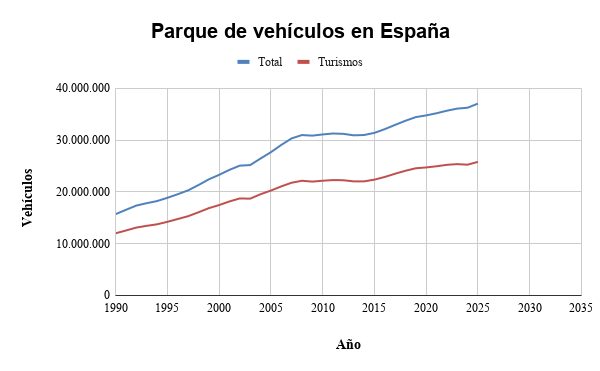
\includegraphics[width=0.8\textwidth]{images/Parque_movil_espana}
  \caption{Evolución del parque de vehículos en España 1990--2025. Fuente: DGT~\cite{dgt2025series}.}
  \label{fig:parque-movil-espana}
\end{figure}

Ese volumen tiene un coste real en tiempo. El informe anual de movilidad urbana de \textit{INRIX}~\cite{inrix2022} estima que los conductores españoles dedican una media de 24 horas al año exclusivamente a buscar aparcamiento. En las grandes ciudades la cifra sube: Madrid, Barcelona y Valencia se sitúan entre las 20 capitales europeas con mayor tiempo de búsqueda. Por ejemplo, en Madrid, los conductores tardan entre 20 y 40 minutos de media en encontrar aparcamiento en zonas céntricas~\cite{parkiduo2025madrid} haciendo que el tiempo en atasco sea de media unas 64 horas.

El aparcamiento regulado en calle y los garajes comerciales reflejan esa presión. En Santa Cruz de Tenerife, el nuevo sistema de zonas azul y verde previsto para 2026~\cite{diariodeavisos2026tarifas} fija tarifas de 1 a 2~€/hora para no residentes en zona azul; los residentes pagarán menos de 1~€/hora o una cuota anual de unos 60~€ en zona verde. En Madrid, el aparcamiento regulado de zona A (SER) alcanza 2,55~€/hora, pero un garaje comercial de centro puede superar los 4,50~€/hora o los 36~€ por 24 horas~\cite{cope2026parking}. En Barcelona, los garajes de máxima demanda superan los 5~€/hora, con jornadas completas en torno a los 30~€~\cite{cope2026parking}.

\begin{table}[H]
  \centering
  \caption{Comparativa de tarifas de aparcamiento regulado por ciudad y zona.}
  \label{tab:tarifas-regulado}
  \begin{tabularx}{\textwidth}{X X c X}
    \toprule
    \textbf{Ciudad}        & \textbf{Zona}       & \textbf{Tarifa (€/hora)} & \textbf{Fuente}       \\
    \midrule
    Santa Cruz de Tenerife & Zona azul (no res.) & 1,00--2,00               & Ayto. Santa Cruz 2026 \\
    Santa Cruz de Tenerife & Zona verde (res.)   & <1,00 / 60\,€/año        & Ayto. Santa Cruz 2026 \\
    Madrid                 & Zona A (SER)        & 2,55                     & EMT / Ayto. Madrid    \\
    Madrid                 & Zona B (SER)        & 1,75                     & EMT / Ayto. Madrid    \\
    Barcelona              & Zona 1 (àrea verda) & 2,75                     & BSM / Ajto. Barcelona \\
    Barcelona              & Zona 2              & 1,40                     & BSM / Ajto. Barcelona \\
    \bottomrule
  \end{tabularx}
\end{table}

\subsection{El mercado en Canarias y el área metropolitana de Tenerife}

Canarias presenta una situación particular. La insularidad limita las alternativas de transporte público y convierte al vehículo privado en la opción dominante para la mayoría de desplazamientos. El Instituto Canario de Estadística~\cite{istac2024} registra en Tenerife una tasa de 870 vehículos por cada 1.000 habitantes en 2025~\cite{eldia2025motoriz} como se puede ver en la \autoref{fig:parque-movil-canarias} siendo esta la más alta del archipiélago, con una edad media del parque superior a los 27~años y más del 13\% de los vehículos superando los 30~años de antigüedad.

La presión sobre el aparcamiento en Santa Cruz de Tenerife y San Cristóbal de La Laguna se explica por la combinación de tres factores: alta densidad residencial en el casco histórico, escasa oferta de aparcamientos públicos subterráneos y concentración de actividad comercial y universitaria. Solo la Universidad de La Laguna, con más de 20.000 estudiantes matriculados, genera una demanda diaria de aparcamiento que actualmente no puede ser absorbida.

A ello se añade la presión normativa ya que la \textit{Ley 7/2021}\footnote{\textbf{Ley 7/2021}: establece la obligatoriedad de las ZBE con carácter vinculante. Santa Cruz de Tenerife (aprox. 210.000 hab.) y San Cristóbal de La Laguna (aprox. 160.000 hab.) quedan dentro de su ámbito de aplicación. La restricción de acceso vehicular no elimina la necesidad de aparcar: la desplaza hacia la periferia, donde la oferta de plazas privadas infrautilizadas es mayor.}, de cambio climático y transición energética~\cite{ley72021}, obliga a los municipios de más de 50.000 habitantes a implantar las ZBE antes del 1 de enero de 2023. Aunque esto se ha ido posponiendo y se prevé que se acabe instaurando en la capital tinerfeña a principios de verano de 2026 haciendo mucho más complicado el acceso al centro urbano de los vehículos antiguos ya mencionados, lo que a su vez incrementa la demanda de aparcamiento en las zonas periféricas.

\begin{figure}[htbp]
  \centering
  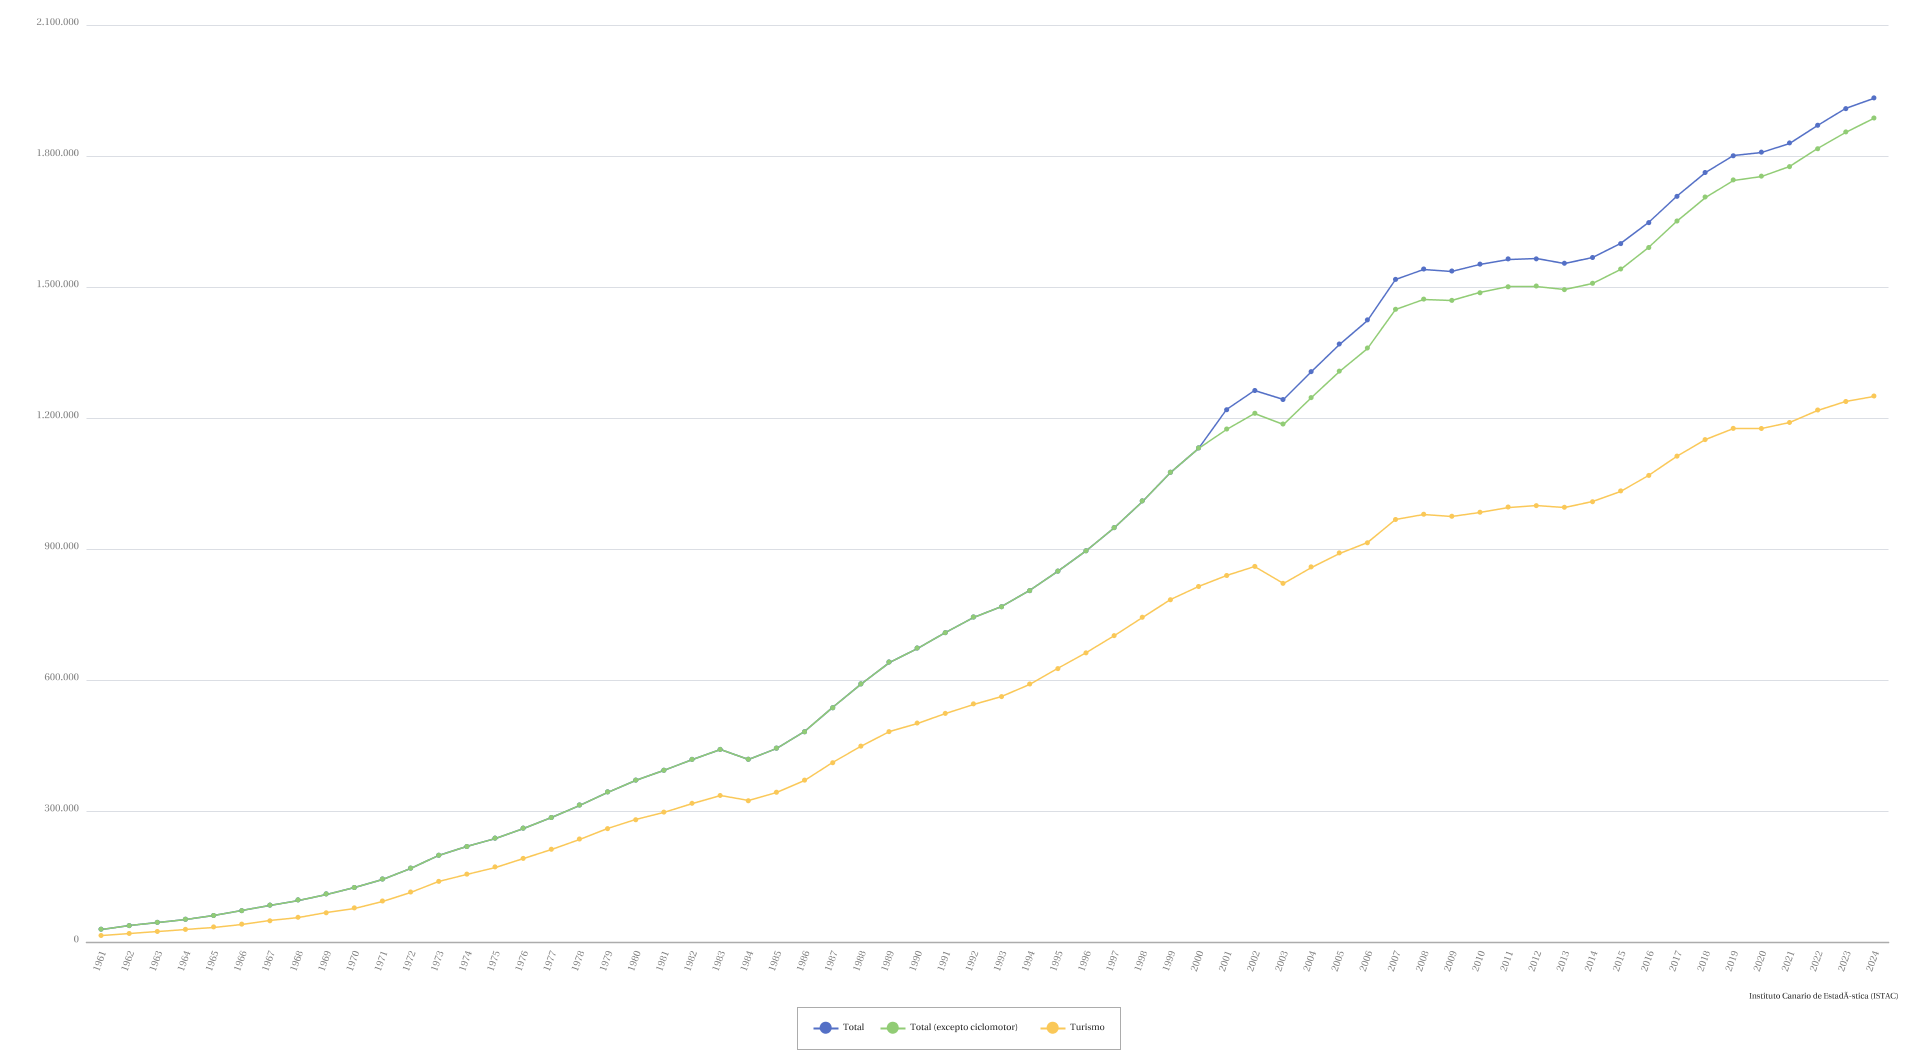
\includegraphics[width=0.9\textwidth]{images/parque_movil_canarias}
  \caption{Evolución anual del parque de vehículos en Canarias (datos desde 1961). Fuente: ISTAC~\cite{istac2024}.}
  \label{fig:parque-movil-canarias}
\end{figure}

\subsection{La Zona de Bajas Emisiones de Santa Cruz de Tenerife}
\label{sec:zbe-sct}

El 13 de abril de 2026, el Ayuntamiento de Santa Cruz de Tenerife aprobó el borrador definitivo de la Ordenanza de Movilidad Sostenible que establece la ZBE municipal~\cite{ayto2026zbe}. La zona abarca 778.244~m\textsuperscript{2} del casco histórico y el distrito Centro, delimitada por la calle Méndez Núñez, la Rambla de Santa Cruz, la avenida de Anaga y el barranco de Santos.

Las restricciones operan de lunes a sábado, de 07:00 a 20:00~horas. Se vetan los vehículos sin etiqueta ambiental DGT: turismos de gasolina matriculados antes de 2001 y diésel anteriores a 2006. La ordenanza prevé 18~meses de carencia para el registro de vehículos y no aplica sanciones efectivas (200~€) hasta 2029.

La normativa contempla una excepción relevante para Parky. Los vehículos con reserva activa en un aparcamiento privado dentro del perímetro quedan exentos de las restricciones ordinarias de acceso. Esta exención convierte a la plataforma en un habilitador de entrada legal al centro urbano, a la vez que redirige la demanda de estacionamiento hacia plazas privadas perimetrales.

\subsection{Disponibilidad y precios en el modelo P2P}

El alquiler de plazas de garaje en Santa Cruz de Tenerife oscila entre 50 y 150~€/mes según ubicación, con la mayor concentración de oferta en el tramo de 60--100~€~\cite{idealista2026garajes} frente a los 7--15~€/día de un parking comercial de rotación. Incluso la tarifa mensual más alta de alquiler resulta competitiva para un conductor que necesita aparcar a diario.

Para el propietario, la relación es igualmente favorable. Una plaza que genera 80~€/mes suma 960~€ anuales por un activo que de otro modo permanece vacío. En mercados donde el modelo P2P ya funciona a escala, JustPark~\cite{justpark2026earnings} documenta entre 500 y 3.000 libras anuales por espacio publicado según la ubicación, lo que da una referencia del potencial del modelo.

La restricción principal del modelo P2P no es de precio, sino de oferta organizada. \textbf{No existe en Canarias ninguna plataforma que agregue esas plazas dispersas, las haga visibles en un mapa y gestione la reserva y el acceso de forma automática.} Esa ausencia define el nicho que Parky busca cubrir.

\section{Objetivos}
\label{sec:objetivos}

\subsection*{Objetivo general}

El objetivo general es diseñar y desarrollar un prototipo funcional de \textit{marketplace P2P} para el alquiler de plazas de aparcamiento privadas en el área metropolitana de Tenerife, que conecte a propietarios de garajes infrautilizados con conductores que necesitan estacionar, y que resuelva de forma integrada la gestión de reservas, el acceso físico al garaje y el flujo de pagos entre particulares.

\subsection*{Objetivos específicos}

\begin{enumerate}

  \item[\textbf{OE1.}] Implementar un sistema de autenticación y control de acceso basado en roles (RBAC)\footnote{\textbf{RBAC} (\textit{Role-Based Access Control}): modelo que asigna permisos a los usuarios según el rol que desempeñan, sin conceder permisos individuales a cada cuenta.} que diferencie la lógica de permisos entre arrendatarios, propietarios y administradores, con soporte para inicio de sesión mediante proveedores externos (OAuth)\footnote{\textbf{OAuth} (\textit{Open Authorization}): protocolo que permite a aplicaciones externas acceder a recursos de un usuario mediante tokens de acceso, sin que este comparta sus credenciales directamente.}.

  \item[\textbf{OE2.}] Construir una \textit{Single Page Application}\footnote{\textbf{SPA} (\textit{Single Page Application}): aplicación web que carga un único documento HTML y actualiza su contenido dinámicamente mediante JavaScript, sin recargar la página desde el servidor.} con enfoque \textit{mobile-first} (ya que la mayoría de reservas se realizan desde móviles) que integre búsqueda sobre mapa interactivo, filtros bidireccionales en tiempo real y geocodificación para el registro de nuevas plazas de aparcamiento.

  \item[\textbf{OE3.}] Garantizar el aislamiento de datos entre usuarios mediante políticas de seguridad (\textit{Row Level Security}, RLS)\footnote{\textbf{RLS} (\textit{Row Level Security}): mecanismo de PostgreSQL que restringe el acceso a filas de una tabla según políticas definidas en el esquema, sin depender de filtros en la capa de aplicación.} aplicadas directamente en el esquema relacional de PostgreSQL.

  \item[\textbf{OE4.}] Prevenir solapamientos en reservas concurrentes mediante \textit{triggers} y procedimientos almacenados en PL/pgSQL, con validación de disponibilidad de plaza ejecutada íntegramente en base de datos, independiente del cliente que origine la petición.

  \item[\textbf{OE5.}] Implementar el flujo de \textit{checkout}, separando automáticamente la tarifa base del arrendador, la comisión de la plataforma y el IGIC del 7\,\% correspondiente a la jurisdicción canaria, y liquidando los pagos directamente a la cuenta bancaria del propietario.

  \item[\textbf{OE6.}] Implementar los estados de reservas mediante rutinas programadas en base a la hora y día actuales, el módulo SmartAccess de apertura remota de garajes con trazabilidad de accesos, y un sistema de valoraciones bidireccionales entre arrendatario y propietario que incentive la confianza en el intercambio entre particulares.

  \item[\textbf{OE7.}] Desplegar la aplicación como cliente web y como aplicación Android nativa desde una base de código TypeScript compartida, utilizando Capacitor\footnote{\textbf{Capacitor}: herramienta de Ionic que empaqueta una aplicación web en un contenedor nativo iOS/Android, dando acceso a las APIs del dispositivo con un único código fuente.} como puente entre la capa web y el sistema operativo móvil.


\end{enumerate}

\chapter{Estudio de tecnologías y decisiones de diseño}
\label{ch:estudio-tecnologias}

Este capítulo describe las tecnologías que componen Parky y justifica cada elección frente a las alternativas consideradas. Para cada herramienta se explica qué función cumple en el sistema, por qué se prefirió sobre las alternativas consideradas y qué compromisos implica la elección.

% ============================================================
\section{Lenguajes de programación y frameworks}
\label{sec:lenguajes}

La arquitectura separa con claridad dos ámbitos: el \textit{frontend}, ejecutado en el navegador o en el dispositivo Android, y el \textit{backend}, delegado íntegramente a servicios externos gestionados. Esta separación permitió concentrar el desarrollo en la lógica de negocio y la experiencia de usuario sin gestionar servidores propios.

% ------------------------------------------------------------
\subsection{Frontend}
\label{subsec:frontend}

El frontend de Parky se organiza en tres capas funcionales: el lenguaje y el sistema de tipos, el framework de renderizado con su cadena de herramientas, y la capa de gestión de datos, formularios y estilos.

\paragraph{Lenguaje y tipado.}
Todo el código fuente está escrito en \textit{TypeScript 5}~\cite{typescript2024} porque su compilador actúa como primera línea de defensa: detecta incompatibilidades de tipo, propiedades inexistentes y posibles valores nulos antes de que el código llegue al navegador. Esta garantía es especialmente valiosa en Parky, donde los errores de tipo tienen consecuencias directas sobre la integridad del negocio. Por ejemplo, una validación incorrecta en el intervalo de reserva puede crear solapamientos, y un error en el desglose de precio base, comisión e IGIC puede generar cargos incorrectos en Stripe. Los componentes de React se expresan en \textit{JSX}\footnote{\textbf{JSX} (\textit{JavaScript XML}): Extensión de sintaxis que permite escribir marcado similar a HTML dentro del código JavaScript.}, y \textit{SWC}\footnote{\textbf{SWC} (\textit{Speedy Web Compiler}): Transpilador escrito en Rust que reemplaza a Babel. Es entre 20 y 70 veces más rápido en compilaciones en frío.} se encarga de transformar ese código a JavaScript puro antes de enviarlo al navegador.

\paragraph{Framework y renderizado.}
La interfaz se construye con \textit{React 18.3.1}~\cite{react2024}. El argumento determinante para elegir esta versión fue el \textit{modo concurrente}: características como \texttt{useTransition} y \texttt{startTransition} permiten marcar como no urgentes las actualizaciones costosas en componentes React —por ejemplo, refrescar el listado de plazas disponibles al mover el mapa— de modo que el motor puede aplazar esa actualización para atender primero los gestos táctiles del usuario, evitando que los paneles de filtros o resultados bloqueen la interacción durante cargas intensivas.

El empaquetador es Vite 6.4.1~\cite{vitejs2024}, que acelera el ciclo de desarrollo al evitar recompilar toda la aplicación ante cada cambio, y optimiza el código para  producción eliminando automáticamente las partes no utilizadas. El enrutado usa \textit{React Router DOM 7}~\cite{reactrouter2024}, configurado con \textit{lazy loading} para cargar el código de cada pantalla únicamente cuando el usuario la visita, lo que reduce el tiempo de carga inicial de la aplicación.

El factor que descartó las alternativas fue la integración con \textit{Capacitor}, el adaptador que empaqueta la aplicación web como APK nativo de Android. Angular quedó descartado por su curva de aprendizaje y menor afinidad con Capacitor; Vue y Svelte ofrecen mejoras de rendimiento notables pero su ecosistema para integraciones híbridas móviles es mucho más reducido. La \autoref{tab:frameworks-comparativa} resume los criterios decisivos:

\begin{table}[htbp]
  \centering
  \caption{Comparativa de frameworks JavaScript de frontend para el desarrollo de Parky.}
  \label{tab:frameworks-comparativa}
  \begin{tabularx}{\textwidth}{lXXXX}
    \toprule
    \textbf{Criterio}        & \textbf{React 18} & \textbf{Vue 3} & \textbf{Angular 17} & \textbf{Svelte 4} \\
    \midrule
    Modo concurrente         & Sí (v18)          & No             & No                  & No                \\
    App nativa (Capacitor)   & Completa          & Limitada       & Limitada            & Experimental      \\
    Ecosistema híbrido móvil & Muy amplio        & Reducido       & Reducido            & Muy reducido      \\
    \bottomrule
  \end{tabularx}
\end{table}

\paragraph{Estado, formularios y estilos.}
La sincronización de datos con el servidor se gestiona con \textit{TanStack Query v5}~\cite{tanstack_query2024}\footnote{\textbf{TanStack Query}: biblioteca de gestión de estado asíncrono que abstrae la caché, el ciclo de vida y la sincronización de datos remotos en aplicaciones React.}, que mantiene la interfaz actualizada automáticamente sin que el desarrollador gestione manualmente cuándo y cómo refrescar los datos. Esto es especialmente relevante en Parky, donde la disponibilidad de una plaza puede cambiar en cualquier momento por una reserva concurrente.

Los formularios (alta de plaza, inicio de sesión, selección de intervalo de reserva) se gestionan con \textit{React Hook Form 7}\footnote{\textbf{React Hook Form}: biblioteca de gestión de formularios que registra los campos mediante refs en lugar de estado de React, minimizando los re-renders durante la edición.}. A diferencia del enfoque estándar de React, los campos no provocan un re-render de la interfaz en cada pulsación de teclado, lo que importa especialmente en formularios con validaciones cruzadas como el selector de intervalo horario de una reserva.

El sistema de estilos usa \textit{Tailwind CSS 4.1.3}~\cite{tailwindcss2024} \footnote{\textbf{Tailwind CSS}: framework de estilos utility-first que compone el diseño visual mediante clases atómicas aplicadas directamente en el marcado, en lugar de hojas CSS por componente.}. Los componentes de interfaz se construyen sobre Radix UI\footnote{\textbf{Radix UI}: biblioteca de componentes primitivos para React que garantiza accesibilidad por defecto sin imponer estilos propios.}, que garantiza un comportamiento accesible por defecto (gestión de foco, navegación por teclado, atributos ARIA, etc.) de modo que Tailwind controla completamente la apariencia visual sin fricciones.

% ------------------------------------------------------------
\subsection{APIs externas de cartografía y geocodificación}
\label{subsec:apis-cartografia}

En Parky la localización geográfica no es un complemento sino el núcleo de la experiencia: el arrendatario busca plazas dentro del área visible del mapa, las visualiza como marcadores geoposicionados y accede a la dirección exacta del garaje. Esto exige dos capacidades independientes: renderizar mapas interactivos y convertir direcciones de texto en coordenadas geográficas.

\paragraph{Leaflet.}
La visualización cartográfica usa \textit{Leaflet 1.9.4}~\cite{leafletjs2024} con el adaptador React-Leaflet 4.2.1. La alternativa natural era la API de \textit{Google Maps}, descartada por su modelo de facturación por volumen. Leaflet es \textit{open source} (bajo licencia BSD-2), sin coste por carga de mapa, y su rendimiento en dispositivos Android de gama media es suficiente para los casos de uso de Parky.

\paragraph{OpenCage Geocoding API.}
La conversión entre direcciones de texto y coordenadas geográficas usa \textit{OpenCage Geocoding API}~\cite{opencage2024}. Este servicio agrega datos de OpenStreetMap, Geonames y otras fuentes abiertas con soporte para direcciones canarias, lo que es fundamental para la aplicación. El plan gratuito incluye 2.500 peticiones diarias, suficiente para el volumen esperado durante la fase de prototipado.

% ------------------------------------------------------------
\subsection{Backend}
\label{subsec:backend}

Se evaluó desarrollar un servidor a medida con \textit{Node.js} o \textit{Python} frente al uso de plataformas \textit{BaaS}\footnote{\textbf{BaaS (Backend-as-a-Service):} Modelo donde un proveedor externo aloja la infraestructura central del servidor —almacenamiento, autenticación, base de datos— y el desarrollador la consume a través de APIs documentadas.}, pero se optó por \textit{Supabase}~\cite{supabase2024} por tres razones.

Supabase cuenta con una capa de autenticación que gestiona el cifrado de contraseñas, los flujos OAuth (Google) de forma nativa y las sesiones mediante \textit{JWT}\footnote{\textbf{JWT} (\textit{JSON Web Token}): estándar RFC 7519 que define un formato compacto para transmitir información entre partes como objeto JSON firmado criptográficamente.}, eliminando la necesidad de implementar y auditar un sistema de identidades propio. También cuenta con un almacenamiento de objetos que gestiona las imágenes de garajes y perfiles con políticas de acceso integradas que impiden que un usuario modifique recursos ajenos. Por último y más importante, para los pagos, la plataforma cuenta con integración con \textit{Stripe Connect}\footnote{\textbf{Stripe Connect}: arquitectura de pagos de Stripe para \textit{marketplaces} que separa y liquida automáticamente los fondos entre las partes.} por medio de Edge Functions, que calculan la comisión de la plataforma, el \textit{IGIC} y transfieren el saldo neto directamente a la cuenta bancaria del propietario del garaje sin que los fondos pasen por una cuenta bancaria central, lo que simplifica la fiscalidad.

Un desarrollo backend propio habría requerido implementar estos tres sistemas desde cero, con la carga de mantenimiento y la superficie de ataque que eso implica en un equipo de una sola persona.

% ------------------------------------------------------------
\subsection{Base de datos}
\label{subsec:bbdd}

Se compararon el modelo relacional y el modelo documental para la capa de persistencia. El dominio de Parky es inherentemente relacional: una reserva vincula a un usuario con una plaza, que pertenece a un garaje, durante un intervalo de tiempo con un pago asociado. \textit{MongoDB}~\cite{mongodb2024} exigiría replicar esa cadena en múltiples documentos, con el riesgo de inconsistencia ante una operación fallida a mitad de ejecución. Es por eso que se eligió \textit{PostgreSQL}~\cite{postgresql2024} porque resuelve esa inconsistencia con integridad referencial mediante \textit{foreign keys}\footnote{\textbf{Foreign key} (clave foránea): columna que referencia la clave primaria de otra tabla, garantizando que no puedan existir reservas de plazas inexistentes o registros huérfanos.} y \textit{transacciones ACID}\footnote{\textbf{ACID}: propiedades de Atomicidad, Consistencia, Aislamiento y Durabilidad que garantizan que las operaciones de base de datos se ejecutan completamente o no se ejecutan en absoluto.}.

Dentro de \textit{PostgreSQL 15} se usan dos características avanzadas: las \textit{políticas RLS} que garantizan que cada usuario solo pueda leer sus propias reservas y los \textit{triggers PL/pgSQL} que comprueban, antes de confirmar cualquier reserva, que no exista solapamiento horario en la misma plaza, manteniendo la consistencia incluso ante peticiones simultáneas.

% ============================================================
\section{Entorno de desarrollo}
\label{sec:entorno}

\paragraph{Editor de código.}
El entorno de desarrollo es \textit{Visual Studio Code}~\cite{vscode2026}. Frente a IDEs\footnote{\textbf{IDE} (\textit{Integrated Development Environment}): entorno que agrupa editor, compilador y depurador en una única aplicación.} basados en IntelliJ, su consumo de memoria es sensiblemente menor, lo que resulta determinante en el desarrollo híbrido con Capacitor, donde el emulador de Android debe estar abierto en paralelo. Además, integra de forma nativa el servidor de TypeScript, por lo que el análisis de tipos en el editor es idéntico al de la compilación real.

\paragraph{Control de versiones.}
El control de versiones usa \textit{Git}~\cite{git2024} con \textit{GitHub}~\cite{github2024} como repositorio remoto. Esta combinación no solo documenta el historial de cambios por fases de desarrollo, sino que actúa como punto de integración con el pipeline de despliegue continuo de Vercel: cada commit en la rama principal desencadena automáticamente un nuevo despliegue en producción.

\paragraph{Diseño de interfaces.}
El diseño visual previo a la implementación se realizó con \textit{Figma}~\cite{figma2024}, que permitió validar la disposición de pantallas, la paleta de colores y las distancias entre elementos antes de traducirlos a clases de Tailwind CSS. Trabajar con un prototipo de alta fidelidad redujo el número de decisiones de diseño durante el desarrollo, concentrando ese esfuerzo en una fase anterior donde el coste de cambio es menor. La figura~\ref{fig:figma-vs-produccion-home} muestra la evolución entre el prototipo inicial y la pantalla principal en producción.

\begin{figure}[H]
  \centering
  \begin{minipage}{0.48\textwidth}
    \centering
    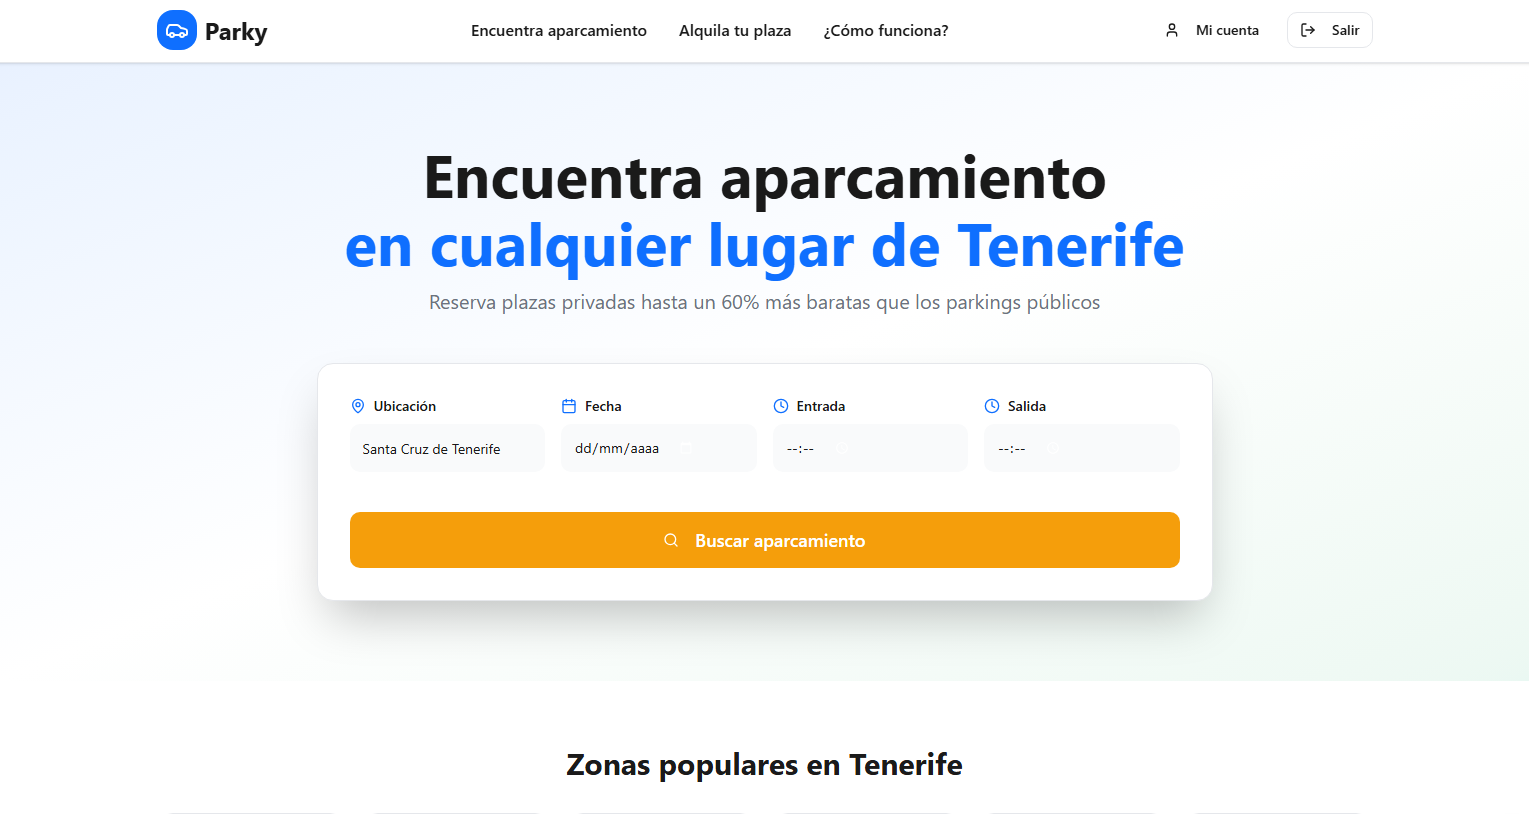
\includegraphics[width=\textwidth]{images/assets/FIGMA_HOME}
  \end{minipage}%
  \hfill
  \begin{minipage}{0.48\textwidth}
    \centering
    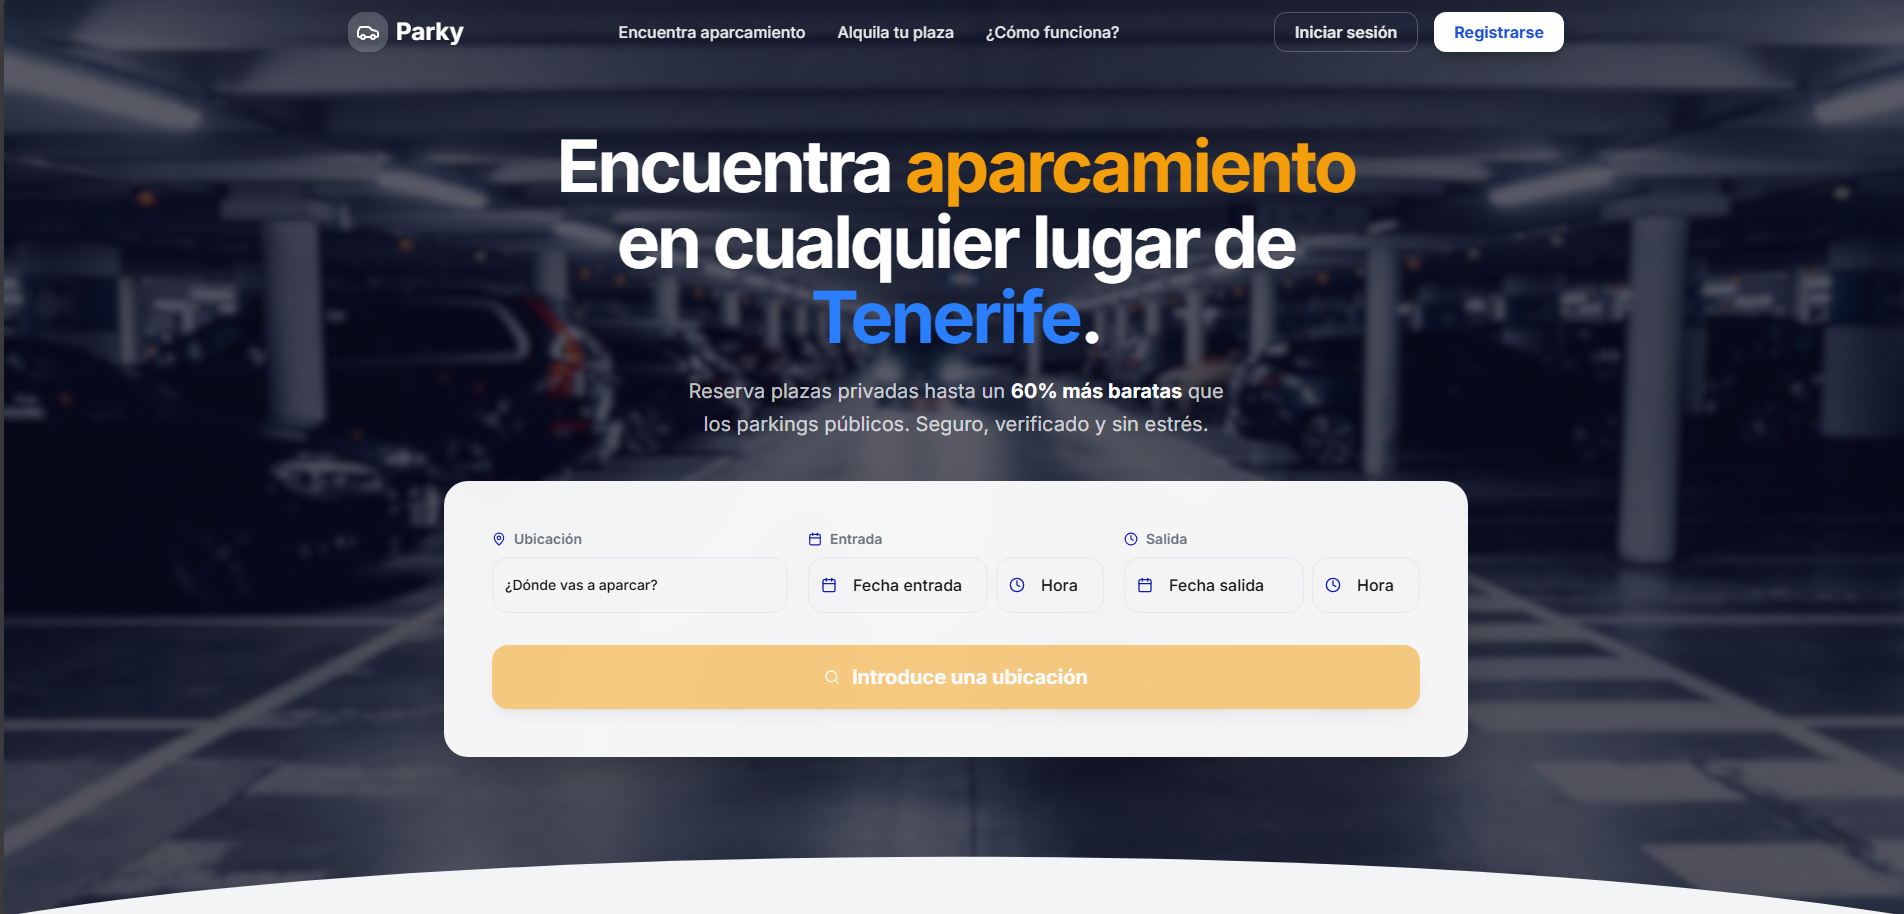
\includegraphics[width=\textwidth]{images/assets/PARKY_HOME}
  \end{minipage}
  \caption{Comparativa entre el prototipo en Figma (izquierda) y la pantalla principal de Parky en producción (derecha).}
  \label{fig:figma-vs-produccion-home}
\end{figure}

% ============================================================
\section{Plataformas de despliegue}
\label{sec:despliegue}

\paragraph{Web: Vercel.}
La versión web se despliega en \textit{Vercel}~\cite{vercel2024}, elegido por su integración nativa con GitHub ya que cada commit en la rama principal desencadena automáticamente una nueva compilación y distribución en su CDN global, sin configuración adicional. Gestiona además los certificados TLS de forma automática. El dominio público de la página se registró en One.com~\cite{onecom2024} y se enlazó a Vercel mediante registros DNS.

\paragraph{Android: Capacitor.}
La aplicación Android se genera con \textit{Capacitor 8.1.0}~\cite{capacitor2024}, que encapsula la aplicación web dentro de una WebView nativa. A diferencia de React Native, que requiere reescribir los componentes en primitivas nativas, Capacitor reutiliza las vistas TypeScript/HTML sin modificaciones, lo que permite mantener una única base de código para web y Android. El APK final se compila desde Android Studio sin modificar ningún componente de React.

% ============================================================
\section{Análisis de alternativas y decisiones de diseño}
\label{sec:dificultades}

La tabla~\ref{tab:baas-comparativa} recoge la comparativa de plataformas BaaS que determinó la elección de Supabase como infraestructura central del proyecto.

\begin{table}[htbp]
  \centering
  \caption{Comparativa de plataformas BaaS frente a las necesidades de Parky.}
  \label{tab:baas-comparativa}
  \begin{tabularx}{\textwidth}{lXXX}
    \toprule
    \textbf{Característica} & \textbf{Supabase}~\cite{supabase2024}
                            & \textbf{Firebase}~\cite{firebase2024}
                            & \textbf{AWS Amplify}~\cite{awsamplify2024} \\
    \midrule
    Motor de base de datos  & PostgreSQL (relacional)
                            & Firestore (documental)
                            & DynamoDB / Aurora Serverless               \\
    Consultas relacionales  & SQL nativo con JOINs
                            & Limitadas, sin JOINs
                            & Posibles con Aurora Serverless             \\
    Row Level Security      & Nativo en PostgreSQL
                            & No disponible
                            & No disponible                              \\
    Autenticación           & Nativo (email, OAuth, MFA)
                            & Authentication integrado
                            & Amazon Cognito                             \\
    Triggers y funciones    & PL/pgSQL + Edge Functions (Deno)
                            & Cloud Functions (externo)
                            & Lambda (externo)                           \\
    Modelo de datos         & Normalizado, tipado
                            & Flexible, sin esquema
                            & Mixto (NoSQL o relacional)                 \\
    Límite tier gratuito    & 500 MB / 2 proyectos
                            & 1 GB (Spark Plan)
                            & 12 meses AWS Free Tier                     \\
    \bottomrule
  \end{tabularx}
\end{table}

Tanto Firebase como AWS Amplify están pensados para modelos de datos documentales y escalan bien en ese contexto, pero el dominio de Parky no encaja ahí. La cadena reserva\,---\,usuario\,---\,plaza\,---\,garaje\,---\,intervalo\,---\,pago se expresa de forma natural en tablas relacionadas mediante JOINs; trasladarla a Firestore obligaría a replicar datos en varios documentos, lo que introduce riesgo de inconsistencia ante cualquier escritura parcial fallida. AWS Amplify ofrece Aurora Serverless como salida relacional, pero su configuración es considerablemente más compleja y carece de RLS nativo, lo que habría obligado a gestionar el aislamiento de datos entre roles desde la capa de aplicación en lugar de resolverlo directamente en el esquema de base de datos.

El principal compromiso de Supabase es su plan gratuito: 500~MB de almacenamiento y pausa automática del proyecto tras 7 días de inactividad. Para un prototipo universitario ambos límites son asumibles, pero una versión comercial requeriría migrar al plan Pro (\$25/mes).
\chapter{Metodología y análisis de requisitos}
\label{ch:metodologia}

Este capítulo establece el marco metodológico del proyecto y formaliza los actores del sistema, los requisitos funcionales y no funcionales, los casos de uso y el diseño de la base de datos.

% ============================================================
\section{Metodología de desarrollo}
\label{sec:metodologia}

El \textit{modelo en cascada}\footnote{\textbf{Modelo en cascada}: Modelo de desarrollo secuencial en el que cada fase (análisis, diseño, desarrollo, pruebas y despliegue) debe cerrarse completamente antes de iniciar la siguiente. Su principal limitación es que asume que los requisitos pueden especificarse en su totalidad antes de escribir una sola línea de código.} fue descartado desde el inicio por una razón estructural importantísima: en un sistema con múltiples capas interdependientes (autenticación, geolocalización, pagos y aplicación nativa) la suposición de que todos los requisitos pueden conocerse antes de implementar es falsa. Especificar completamente el sistema antes de construirlo habría sido imposible en Parky, y tres episodios durante el desarrollo lo demuestran.

En primer lugar, el módulo \textit{SmartAccess} no figuraba en el análisis inicial y emergió en el sprint~4 porque al construir el flujo de reservas quedó claro que «el arrendatario llega al garaje y no puede entrar» era exactamente la fricción central que la plataforma pretendía eliminar. En segundo lugar, el \textit{trigger} de solapamiento de reservas se añadió en el sprint~8, no al principio ya que solo al implementar el flujo completo se hizo evidente que dos usuarios podían reservar la misma plaza simultáneamente. En tercer lugar, la auditoría de seguridad del sprint~7 detectó que el diseño de borrado de reservas destruía el historial financiero de los arrendadores, algo que solo resulta visible cuando el sistema maneja datos reales. En cascada, cualquiera de estos tres hallazgos habría obligado a reabrir la fase de requisitos y rediseñar desde arriba, con un coste de retroceso enorme.

Por ello se adoptó \textbf{Scrum}~\cite{scrum2020}\footnote{\textbf{Scrum}: Marco de trabajo ágil definido por Schwaber y Sutherland~\cite{scrum2020} que organiza el desarrollo en iteraciones de duración fija llamadas \textit{sprints}, al término de cada una de las cuales se entrega un incremento funcional del producto.} con \textit{sprints}\footnote{\textbf{Sprints}: Iteración de duración fija (dos semanas en Parky) al final de la cual se revisa el trabajo entregado, se ajusta el \textit{backlog} y se reprioriza el siguiente ciclo.} de dos semanas, cada uno centrado en un módulo de alto nivel. Scrum acepta que los requisitos evolucionan y lo convierte en una ventaja en lugar de un problema de modo que los errores que se detectan al final de cada ciclo, se corrigen en el siguiente sin afectar lo ya construido. Al tratarse de un proyecto unipersonal, los tres roles canónicos del marco (\textit{Product Owner}, \textit{Scrum Master} y equipo de desarrollo) convergieron en una única persona, y la retrospectiva de cada ciclo fue el mecanismo principal para detectar \textit{deuda técnica}\footnote{\textbf{Deuda técnica}: Coste futuro de corrección acumulado al tomar decisiones de implementación rápidas en lugar de óptimas. En un proyecto unipersonal, la retrospectiva de sprint es el único mecanismo formal para identificarla antes de que se propague.} antes de que se acumulara.

La Tabla~\ref{tab:sprints} recoge los nueve sprints en los que se desarrolló el prototipo, con sus respectivos módulos principales y entregables.

\begin{table}[h]
  \centering
  \caption{Sprints de desarrollo de Parky (enero--mayo de 2026).}
  \label{tab:sprints}
  \begin{tabularx}{\textwidth}{clXX}
    \toprule
    \textbf{Sprint} & \textbf{Período}    & \textbf{Módulo principal}
                    & \textbf{Entregable}                                                             \\
    \midrule
    \rowcolor{gray!5}
    1               & 6--19 ene           & Infraestructura base          & Scaffolding React/Vite,
    autenticación Supabase, rutas protegidas y modo oscuro.                                           \\
    2               & 20 ene--2 feb       & Modelo de datos y perfil      & Esquema de base de datos,
    RLS básico, edición de perfil e imágenes en Storage.                                              \\
    \rowcolor{gray!5}
    3               & 3--16 feb           & Plazas y mapa                 & Integración Leaflet,
    CRUD de garajes y plazas, React Query como capa de caché.                                         \\
    4               & 17 feb--2 mar       & Reservas, SmartAccess y pagos & Motor de precios, módulo
    SmartAccess con log de accesos y arquitectura de pagos.                                           \\
    \rowcolor{gray!5}
    5               & 3--16 mar           & Despliegue multiplataforma    & Vercel, compilación
    Android con Capacitor y APK nativo.                                                               \\
    6               & 17 mar--26 abr      & Memoria del TFG               & Redacción de los
    capítulos 1 a 4; commits de código suspendidos.                                                   \\
    \rowcolor{gray!5}
    7               & 27 abr--10 may      & Seguridad y calidad           & Auditoría de RLS,
    borrado lógico en \texttt{bookings} y HSTS/CSP en Vercel.                                         \\
    8               & 10--14 may          & Disponibilidad y reserva      & Horarios recurrentes,
    trigger de solapamiento y buffer de 15 minutos.                                                   \\
    \rowcolor{gray!5}
    9               & 15--19 may          & Pulido UX                     & \textit{Code splitting}
    (reducción del 95\,\% del \textit{bundle}), navegación inferior y
    \textit{touch targets} móvil.                                                                     \\
    \bottomrule
  \end{tabularx}
\end{table}

% ============================================================
\section{Actores del sistema}
\label{sec:actores}

En cuanto a los actores del sistema, Parky define cuatro roles principales definidos con claridad en la tabla~\ref{tab:actores-principales}. La separación entre arrendador y arrendatario no es solo conceptual sino también funcional, porque cada rol queda restringido a un subconjunto de datos distinto impuesto por las políticas RLS de la base de datos.

\begin{table}[H]
  \centering
  \caption{Actores del sistema Parky.}
  \label{tab:actores-principales}
  \begin{tabularx}{\textwidth}{lX}
    \toprule
    \textbf{Actor} & \textbf{Responsabilidades y alcance}                                                                                                                                             \\
    \midrule
    \rowcolor{gray!5}
    Arrendador     & Propietario de garajes. Publica plazas con precio, fotos y geolocalización. Acepta o rechaza reservas entrantes. Recibe pagos a través de Stripe Connect.                        \\
    \\
    Arrendatario   & Conductor que alquila plazas. Busca en el mapa, reserva, paga con Stripe y valora la plaza al finalizar.                                                                         \\
    \\
    \rowcolor{gray!5}
    Administrador  & Opera desde el \textit{dashboard} de Supabase con privilegios de servicio. Suspende cuentas, corrige datos y ejecuta consultas de mantenimiento. Sin interfaz en el cliente web. \\
    \\
    Sistema        & Componente automatizado. Procesa transacciones (Stripe), geocodifica direcciones (OpenCage), gestiona sesiones (OAuth) y emite notificaciones almacenadas en base de datos.      \\
    \bottomrule
  \end{tabularx}
\end{table}

% ============================================================
\section{Requisitos funcionales}
\label{sec:requisitos_funcionales}

Los requisitos funcionales se construyeron a partir de los objetivos específicos OE1--OE7 definidos en el capítulo introductorio dentro de la sección \ref*{sec:objetivos} y de un análisis de las funcionalidades de plataformas P2P de referencia. El prototipo final cubre los dieciséis requisitos funcionales listados en la Tabla~\ref{tab:rf}, con la salvedad de que RF-08 y RF-16 están implementados a nivel de arquitectura y modelo de datos pero sin procesar cobros reales, al tratarse de un prototipo académico y que no es necesario el cobro para mostrar la funcionalidad. Los dieciséis requisitos funcionales se agrupan por módulo en la Tabla~\ref{tab:rf}:

\begin{table}[htbp]
  \centering
  \caption{Requisitos funcionales de Parky.}
  \label{tab:rf}
  \begin{tabularx}{\textwidth}{llX}
    \toprule
    \textbf{ID} & \textbf{Actor}            & \textbf{Descripción}                                                                                                                                                                                                                                                                      \\
    \midrule
    \rowcolor{gray!5}
    RF-01       & Arr. / Arrend. / Admin.   & Registro e inicio de sesión mediante email/contraseña y OAuth~(Google).                                                                                                                                                                                                                   \\
    RF-02       & Arrendador / Arrendatario & El sistema asigna automáticamente el rol \textit{Arrendatario} al registrar al usuario; al crear su primer garaje, el perfil adquiere también el rol \textit{Arrendador}, quedando ambos activos simultáneamente en la misma cuenta.                                                      \\
    \rowcolor{gray!5}
    RF-03       & Arrendador                & Dar de alta un garaje con nombre, dirección y fotos, y gestionar sus plazas individuales (crear, editar, desactivar) fijando precio por hora y disponibilidad.                                                                                                                            \\
    RF-04       & Arrendatario              & Visualizar plazas disponibles en el mapa dentro del área visible y filtrarlas por precio y horario.                                                                                                                                                                                       \\
    \rowcolor{gray!5}
    RF-05       & Arrendatario              & Solicitar reserva sobre una plaza con fecha y hora de inicio y fin.                                                                                                                                                                                                                       \\
    RF-06       & Sistema                   & Rechazar reservas que solapen con otra confirmada o en curso en la misma plaza.                                                                                                                                                                                                           \\
    \rowcolor{gray!5}
    RF-07       & Arrendador                & Las reservas entrantes permanecen en estado \texttt{pendiente} hasta su confirmación o rechazo manual.                                                                                                                                                                                    \\
    RF-08       & Sistema                   & Calcular el importe del cobro con desglose de comisión de plataforma e IGIC (7\,\%), y registrar la transacción en el modelo de datos de pagos. La integración con la API de Stripe Connect para procesar cobros reales está prevista para la versión comercial (véase \textit{roadmap}). \\
    \rowcolor{gray!5}
    RF-09       & Sistema                   & Reembolsar íntegramente al arrendatario si la reserva se cancela antes del inicio.                                                                                                                                                                                                        \\
    RF-10       & Arrendatario              & Valorar una plaza de 1 a~5 únicamente si la reserva está en estado \texttt{completada}.                                                                                                                                                                                                   \\
    \rowcolor{gray!5}
    RF-11       & Sistema                   & Notificar al arrendador cuando llegue una nueva solicitud de reserva.                                                                                                                                                                                                                     \\
    RF-12       & Sistema                   & Notificar al arrendatario cuando el arrendador confirme o rechace su reserva.                                                                                                                                                                                                             \\
    \rowcolor{gray!5}
    RF-13       & Arrendador / Arrendatario & Editar nombre, fotografía de perfil y datos de contacto propios.                                                                                                                                                                                                                          \\
    RF-14       & Arrendador / Arrendatario & Consultar el historial de reservas propias con estado, fecha e importe.                                                                                                                                                                                                                   \\
    \rowcolor{gray!5}
    RF-15       & Sistema                   & Generar un código QR único para cada reserva confirmada, válido únicamente durante la ventana temporal activa (SmartAccess).                                                                                                                                                              \\
    RF-16       & Arrendador                & Completar el alta en Stripe Connect para vincular una cuenta bancaria y habilitar la recepción de transferencias. Previsto para la versión comercial.                                                                                                                                     \\
    \bottomrule
  \end{tabularx}
\end{table}

% ============================================================
\section{Requisitos no funcionales}
\label{sec:requisitos_no_funcionales}

Los requisitos no funcionales establecen los criterios de calidad que el sistema debe satisfacer con independencia de las funcionalidades concretas, y se pueden ver en la tabla \ref{tab:rnf}. El criterio de rendimiento responde a un dato práctico, ya que los usuarios de Parky consultan el mapa mientras circulan por la ciudad y una respuesta superior a tres segundos en condiciones de conectividad habituales provoca el abandono antes de completar la búsqueda. El diseño se adapta a resoluciones de gama media porque ese es el perfil de dispositivo predominante entre los conductores que buscan aparcamiento en Tenerife, y la misma base de código React compila sin modificaciones como aplicación nativa de Android, lo que cubre el requisito de portabilidad sin duplicar el desarrollo. La disponibilidad del servicio se apoya en las garantías de Vercel y Supabase, cuya infraestructura redundante sería inviable de replicar con un servidor propio a este coste de proyecto.

\begin{table}[htbp]
  \centering
  \caption{Requisitos no funcionales de Parky.}
  \label{tab:rnf}
  \begin{tabularx}{\textwidth}{lX}
    \toprule
    \textbf{Categoría} & \textbf{Criterio}                                                                                                                                                                                                       \\
    \midrule
    \rowcolor{gray!5}
    Rendimiento        & \textit{LCP}\footnote{\textbf{LCP} (Large Contentful Paint): mide el tiempo que tarda en renderizarse el elemento de contenido más grande visible de una página} inferior a 3~s bajo conectividad 4G de latencia media. \\
    Seguridad          & Todas las tablas tienen RLS activo. Cada petición al backend se valida con JWT. Ninguna clave secreta se expone en el cliente.                                                                                          \\
    \rowcolor{gray!5}
    Usabilidad         & Diseño \textit{mobile-first} con punto de ruptura desde 375~px.                                                                                                                                                         \\
    Portabilidad       & La base de código React compila como APK para Android mediante Capacitor sin modificar componentes.                                                                                                                     \\
    \rowcolor{gray!5}
    Disponibilidad     & Vercel y Supabase garantizan un \textit{uptime} del 99,5~\% en sus SLA.                                                                                                                                                 \\
    Mantenibilidad     & El código fuente sigue convenciones de tipado estrictas verificadas en cada compilación, lo que reduce la probabilidad de errores silenciosos antes de llegar a producción.                                             \\
    \bottomrule
  \end{tabularx}
\end{table}

% ============================================================
\section{Modelo de casos de uso}
\label{sec:casos_de_uso}

El modelo de casos de uso describe las interacciones entre los cuatro actores del sistema y las funcionalidades que Parky expone. El diagrama de la Figura~\ref{fig:casos_de_uso_uml} organiza estos casos de uso por módulo funcional, y las tablas siguientes detallan los cuatro de mayor peso con sus precondiciones, postcondiciones y flujos alternativos.

% ------------------------------------------------------------
\begin{table}[H]
  \centering
  \caption{CU-01: Autenticarse y obtener rol.}
  \label{tab:cu-01}
  \begin{tabularx}{\textwidth}{|>{\columncolor{gray!15}\bfseries}l|X|}
    \hline
    ID y Nombre       & CU-01: Autenticarse y obtener rol                                                                                                             \\ \hline
    Actor             & Todos                                                                                                                                             \\ \hline
    Precondición      & Sin sesión activa.                                                                                                                                \\ \hline
    Postcondición     & JWT activo y rol almacenado en \texttt{profiles}.                                                                                                 \\ \hline
    Flujo principal   &
    \begin{itemize}[leftmargin=3mm, itemsep=0mm, topsep=1mm]
      \item[1.] El usuario accede a la pantalla de autenticación.
      \item[2.] Se autentica con email/contraseña o Google OAuth.
      \item[3.] El sistema asigna automáticamente el rol Arrendatario; si el usuario crea un garaje posteriormente, el perfil asciende a Arrendador sin intervención manual.
      \item[4.] El rol se persiste en \texttt{profiles}.
      \item[5.] El sistema redirige al \textit{dashboard} correspondiente.
    \end{itemize} \\ \hline
    Flujo alternativo & Si el proveedor OAuth devuelve error, se ofrece reintento o autenticación con email/contraseña.                                                   \\ \hline
  \end{tabularx}
\end{table}

\begin{table}[H]
  \centering
  \caption{CU-02: Publicar plaza de garaje.}
  \label{tab:cu-02}
  \begin{tabularx}{\textwidth}{|>{\columncolor{gray!15}\bfseries}l|X|}
    \hline
    ID y Nombre       & CU-02: Publicar plaza de garaje                                                                                             \\ \hline
    Actor             & Arrendador                                                                                                                  \\ \hline
    Precondición      & Sesión activa con rol \texttt{arrendador}.                                                                                  \\ \hline
    Postcondición     & Plaza registrada y visible en el mapa.                                                                                      \\ \hline
    Flujo principal   &
    \begin{itemize}[leftmargin=3mm, itemsep=0mm, topsep=1mm]
      \item[1.] El arrendador accede al formulario de alta de plaza.
      \item[2.] Introduce descripción, precio por hora y fotos.
      \item[3.] Confirma la posición geográfica sobre el mapa interactivo.
      \item[4.] El cliente ejecuta una inserción en la API REST de Supabase.
      \item[5.] El sistema confirma el alta y actualiza el mapa.
    \end{itemize}                                                                           \\ \hline
    Flujo alternativo & Si la subida de imágenes al \textit{bucket} de Supabase Storage falla, el registro no se persiste y se notifica al usuario. \\ \hline
  \end{tabularx}
\end{table}

\begin{table}[H]
  \centering
  \caption{CU-03: Buscar y filtrar plazas en el mapa.}
  \label{tab:cu-03}
  \begin{tabularx}{\textwidth}{|>{\columncolor{gray!15}\bfseries}l|X|}
    \hline
    ID y Nombre       & CU-03: Buscar y filtrar plazas                                                                          \\ \hline
    Actor             & Arrendatario                                                                                            \\ \hline
    Precondición      & Sesión activa y permisos de geolocalización concedidos.                                                 \\ \hline
    Postcondición     & Mapa con marcadores de plazas activas en el área visible.                                               \\ \hline
    Flujo principal   &
    \begin{itemize}[leftmargin=3mm, itemsep=0mm, topsep=1mm]
      \item[1.] La aplicación obtiene la posición GPS del dispositivo.
      \item[2.] Se consultan plazas en estado \texttt{activo} dentro del bounding box visible.
      \item[3.] El usuario filtra por precio máximo o rango horario.
      \item[4.] Al pulsar un marcador se muestra la ficha con precio y disponibilidad.
    \end{itemize}                                     \\ \hline
    Flujo alternativo & Sin GPS disponible, el usuario introduce una dirección que OpenCage Geocoding convierte en coordenadas. \\ \hline
  \end{tabularx}
\end{table}

\begin{table}[H]
  \centering
  \caption{CU-04: Realizar reserva y pago.}
  \label{tab:cu-04}
  \begin{tabularx}{\textwidth}{|>{\columncolor{gray!15}\bfseries}l|X|}
    \hline
    ID y Nombre       & CU-04: Realizar reserva y pago                                                                          \\ \hline
    Actor             & Arrendatario                                                                                            \\ \hline
    Precondición      & Sesión activa y plaza seleccionada.                                                                     \\ \hline
    Postcondición     & Reserva en estado \texttt{pendiente}; intervalo horario bloqueado.                                      \\ \hline
    Flujo principal   &
    \begin{itemize}[leftmargin=3mm, itemsep=0mm, topsep=1mm]
      \item[1.] El arrendatario selecciona fecha, hora de inicio y hora de fin.
      \item[2.] El trigger PL/pgSQL verifica que no exista solapamiento en la misma plaza.
      \item[3.] El usuario introduce los datos de tarjeta en el formulario de Stripe.
      \item[4.] Stripe confirma el cargo y la reserva avanza a estado \texttt{pendiente}.
      \item[5.] Ambas partes reciben notificación del cambio de estado.
    \end{itemize}                                         \\ \hline
    Flujo alternativo & Si la tarjeta es rechazada o el pago expira, la reserva no se persiste y la plaza permanece disponible. \\ \hline
  \end{tabularx}
\end{table}

\begin{figure}[H]
  \centering
  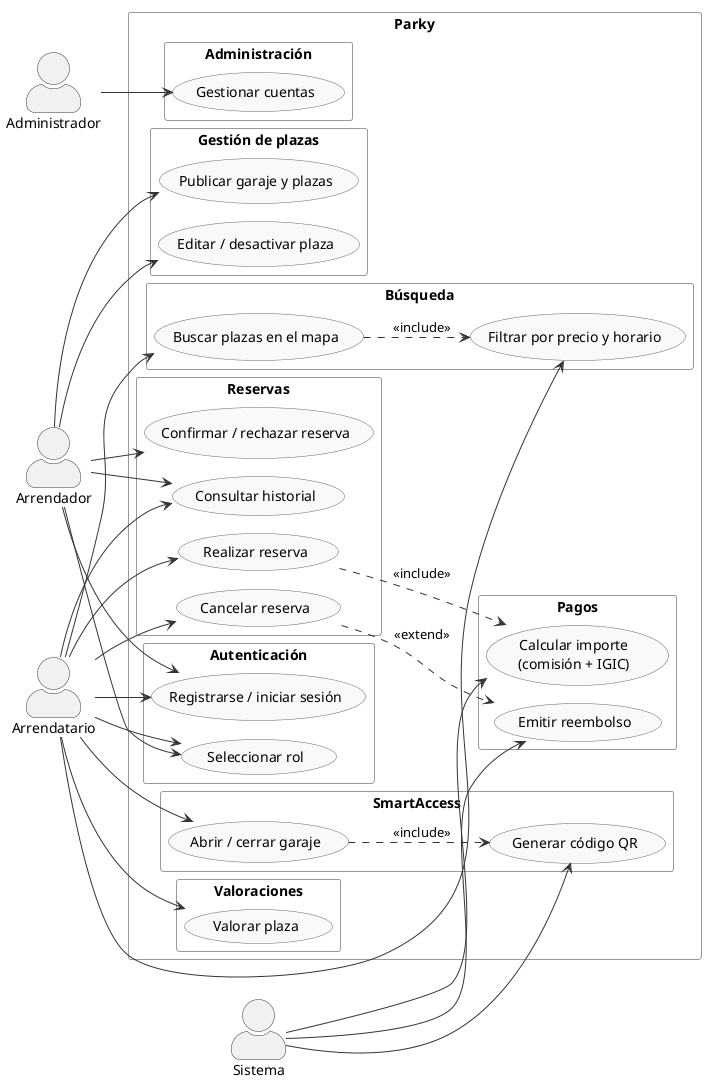
\includegraphics[width=0.48\textwidth]{images/assets/casos_de_uso}
  \caption{Diagrama de casos de uso del sistema Parky.}
  \label{fig:casos_de_uso_uml}
\end{figure}

% ============================================================
\section{Trazabilidad de objetivos}
\label{sec:trazabilidad}
% ============================================================

La Tabla~\ref{tab:trazabilidad} recoge la correspondencia entre los objetivos específicos de la sección~\ref{sec:objetivos}, los requisitos funcionales de la Tabla~\ref{tab:rf} y los casos de uso de la sección~\ref{sec:casos_de_uso}, mostrando que todos los objetivos quedan cubiertos por al menos un requisito y un caso de uso verificable.

\begin{table}[htbp]
  \centering
  \caption{Matriz de trazabilidad: objetivo específico \textrightarrow\ req. funcional \textrightarrow\ caso de uso.}
  \label{tab:trazabilidad}
  \begin{tabularx}{\textwidth}{lXX}
    \toprule
    \textbf{Objetivo}                         & \textbf{Req. funcionales}                                   & \textbf{Casos de uso} \\
    \midrule
    \rowcolor{gray!5}
    OE1 — Autenticación y RBAC                & RF-01, RF-02                                                & CU-01                 \\
    OE2 — SPA, mapa y geocodificación         & RF-03, RF-04, RF-13                                         & CU-02, CU-03          \\
    \rowcolor{gray!5}
    OE3 — Aislamiento RLS                     & RF-03 a RF-15 (operaciones sobre datos propios de cada rol) & CU-01 a CU-04         \\
    OE4 — Integridad de reservas              & RF-05, RF-06                                                & CU-04                 \\
    \rowcolor{gray!5}
    OE5 — \textit{Checkout} e IGIC            & RF-08, RF-09                                                & CU-04                 \\
    OE6 — Estados, SmartAccess y valoraciones & RF-07, RF-10, RF-11, RF-12, RF-14, RF-15                    & CU-04                 \\
    \rowcolor{gray!5}
    OE7 — Despliegue web y Android            & RF-01 a RF-16                                               & CU-01 a CU-04         \\
    \bottomrule
  \end{tabularx}
\end{table}

% ============================================================
\section{Diseño de la base de datos}
\label{sec:diseno-bd}

La base de datos se ejecuta sobre PostgreSQL~15 en Supabase. El esquema normaliza cada entidad de negocio en tablas independientes vinculadas por \textit{foreign keys}. La tabla \texttt{profiles} almacena la información de cada usuario, incluyendo su rol (arrendador o arrendatario) y datos de contacto. La tabla \texttt{garages} representa los garajes publicados por los arrendadores, con su dirección y geolocalización. Cada garaje puede tener varias plazas, por lo que se almacenan en la tabla \texttt{parking\_spots}, que incluye precio por hora y disponibilidad y se relaciona con \texttt{garages} mediante una \textit{foreign key}. Las reservas se registran en la tabla \texttt{bookings} con su estado y ventana temporal, mientras que las valoraciones de los arrendatarios se almacenan en la tabla \texttt{reviews}. El modelo de pagos se apoya en la tabla \texttt{transactions}, que registra el importe, comisión e IGIC de cada reserva confirmada.

% ------------------------------------------------------------
% ------------------------------------------------------------
\subsection{Diagrama de la base de datos}
\label{subsec:diagramas}

\begin{figure}[H]
  \centering
  \hspace*{-6cm}
  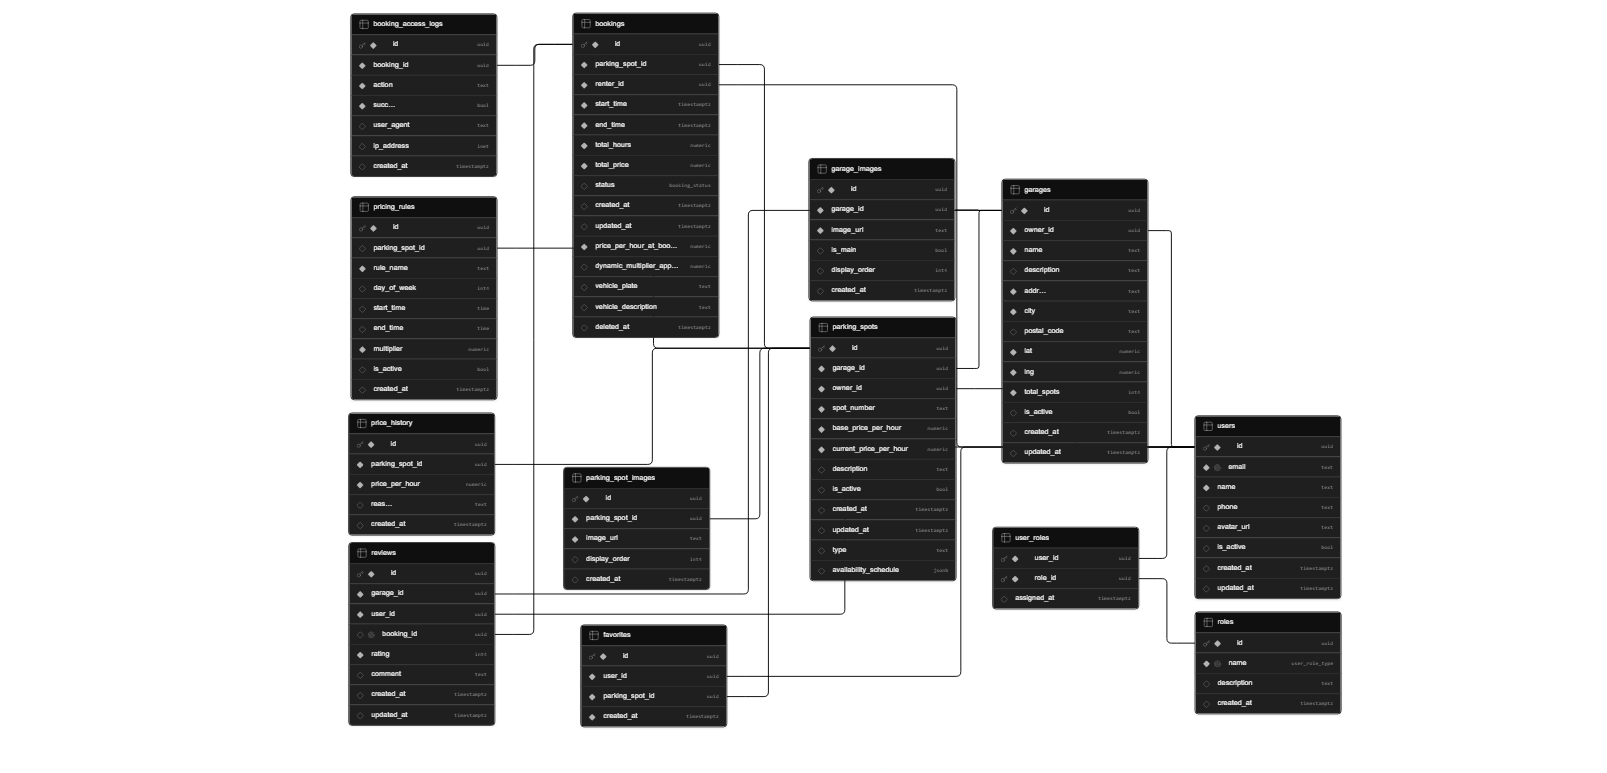
\includegraphics[width=1.15\textheight,keepaspectratio]{images/assets/Diagrama_ER}
  \caption{Diagrama entidad-relación del esquema de base de datos de Parky.}
  \label{fig:er-diagram}
\end{figure}

% ------------------------------------------------------------
\subsection{Políticas RLS}
\label{subsec:rls}

Las políticas de \textit{Row Level Security} (RLS) de PostgreSQL filtran automáticamente las filas que cada usuario puede leer o modificar antes de devolver cualquier resultado, sin que el código del cliente intervenga. Esto significa que aunque un arrendatario manipulara la petición para incluir el identificador de otro usuario, la base de datos rechazaría la operación sin necesidad de ninguna validación adicional en el servidor de aplicación. Las cuatro políticas principales de Parky se recogen en la Tabla~\ref{tab:rls-policies}: cada una vincula el acceso a la identidad autenticada mediante \texttt{auth.uid()}, de modo que arrendadores y arrendatarios operan sobre subconjuntos de datos completamente aislados entre sí.

\begin{table}[htbp]
  \centering
  \caption{Políticas de seguridad a nivel de fila (RLS) del esquema de Parky.}
  \label{tab:rls-policies}
  \begin{tabularx}{\textwidth}{llX}
    \toprule
    \textbf{Tabla}    & \textbf{Operación} & \textbf{Condición de acceso}                                                                                       \\
    \midrule
    \rowcolor{gray!5}
    \texttt{profiles} & SELECT, UPDATE     & Solo el propio usuario puede leer o modificar su perfil (\texttt{auth.uid() = user\_id}).                          \\
    \texttt{bookings} & SELECT             & Arrendador: ve reservas de sus plazas. Arrendatario: solo sus propias reservas (\texttt{tenant\_id = auth.uid()}). \\
    \rowcolor{gray!5}
    \texttt{bookings} & INSERT             & Solo usuarios con rol \texttt{arrendatario} pueden crear reservas a su nombre.                                     \\
    \texttt{reviews}  & INSERT             & Solo si la reserva referenciada pertenece al usuario y está en estado \texttt{completada}.                         \\
    \bottomrule
  \end{tabularx}
\end{table}

% ------------------------------------------------------------
\subsection{Trigger de integridad de reservas}
\label{subsec:triggers}

La tabla \texttt{bookings} está protegida por dos triggers que garantizan la integridad de las reservas a nivel de base de datos. El primero, \texttt{prevent\_booking\_overlap}, impide que se creen dos reservas solapadas en la misma plaza: antes de evaluar el solapamiento, el trigger adquiere un bloqueo explícito sobre la fila de \texttt{parking\_spots} correspondiente mediante \texttt{SELECT \ldots FOR UPDATE}, serializando el acceso concurrente a la misma plaza y garantizando que dos transacciones simultáneas no pasan el chequeo de forma simultánea bajo el nivel de aislamiento \texttt{READ COMMITTED} que PostgreSQL usa por defecto. Adicionalmente, aplica un espaciado de 15 minutos entre reservas consecutivas (con el fin de garantizar el tiempo necesario a sacar el coche o en su defecto a la grúa). El segundo, \texttt{enforce\_booking\_status\_machine}, restringe las transiciones del estado de la reserva a la secuencia \texttt{pendiente} $\to$ \texttt{confirmada} $\to$ \texttt{activa} $\to$ \texttt{completada}, impidiendo que una reserva cancelada pueda reactivarse.


PostgreSQL permite una alternativa para detectar solapamientos temporales mediante restricciones \texttt{EXCLUDE} con rangos de tipo \texttt{tstzrange} e índices GiST. Esta opción fue considerada y descartada por dos razones. La primera es que las restricciones \texttt{EXCLUDE} se limitan a comparar rangos y no admiten lógica adicional dentro de la misma expresión, de modo que incorporar el buffer de 15 minutos habría requerido una función de comparación personalizada, añadiendo complejidad sin beneficio claro. La segunda es que el trigger produce mensajes de error estructurados que la capa de aplicación puede interpretar directamente para mostrar al conductor el motivo del rechazo, mientras que una violación de restricción \texttt{EXCLUDE} devuelve un error genérico de integridad referencial.

\chapter{Estudio de viabilidad económica}
\label{ch:viabilidad_economica}

En esta sección, se llevará a cabo un análisis detallado de la viabilidad económica asociada con la implementación del sistema Parky. Este estudio se ha diseñado bajo la premisa de la ejecución del proyecto en un entorno empresarial profesional real, haciendo uso de recursos humanos cualificados en el sector tecnológico y proyectado al mercado del año 2026. El objetivo es corroborar que, más allá de la solidez técnica, el proyecto es escalable, sostenible y rentable económicamente a medio plazo, elaborando asimismo un esquema integral de comercialización, mantenimiento y proyecciones de retorno.

\section{Desarrollo del proyecto}
\label{sec:desarrollo_proyecto}

Para garantizar un proceso de creación eficiente y cumplir con los más altos estándares de calidad propios de una plataforma P2P\footnote{\textit{Peer-to-Peer}: Red entre pares que permite el intercambio de información y servicios directos entre usuarios, sin intermediación bancaria o administrativa central en transacciones puras.} transaccional, el ciclo de vida del proyecto se ha dividido en seis fases bien definidas. La adopción de un modelo iterativo e incremental ha permitido paralelizar tareas críticas, acortando los tiempos generales del proyecto.

\begin{itemize}
    \item \textbf{Análisis (27 días):} Fase crítica centrada en la definición exhaustiva de requisitos funcionales, validación de la lógica de negocio del modelo de aparcamiento y análisis normativo en torno a las ZBE\footnote{Zonas de Bajas Emisiones (ZBE): Áreas urbanas específicas con restricciones de acceso vehiculares para mejorar la calidad del aire.}. Es indispensable afianzar estos conceptos para evitar sobrecostes en etapas posteriores.
    \item \textbf{Diseño (24 días):} Establecimiento de la arquitectura del software. En esta etapa se decide el ecosistema tecnológico (React, TypeScript, Supabase, Capacitor), la estructuración de la base de datos PostgreSQL en cumplimiento estricto con las políticas de RLS\footnote{\textit{Row Level Security} (RLS): Políticas de base de datos que restringen qué filas de una tabla pueden ser leídas o manipuladas por un usuario determinado.} y el diseño de interfaces UI/UX\footnote{\textit{User Interface / User Experience} (UI/UX): Diseño centrado en la interacción del usuario y la percepción visual de la plataforma.} para las plataformas web y móvil.
    \item \textbf{Desarrollo e implementación (135 días):} Constituye la actividad central del cronograma. Durante estos meses, se ejecuta la codificación del \textit{frontend}, la construcción de la base de datos y la orquestación del \textit{backend}, destacando la integración de la pasarela de pagos descentralizada con Stripe Connect y la geolocalización mediante Leaflet.
    \item \textbf{Pruebas (130 días):} Dada la sensibilidad en el procesamiento de transacciones financieras, esta fase, ejecutada en paralelo al desarrollo, resulta innegociable. Engloba pruebas unitarias, de integración y simulaciones de vulnerabilidad, garantizando que el reparto de comisiones y el cálculo de la tarifa tributaria operan sin fallos.
    \item \textbf{Despliegue (10 días):} Fase de paso técnico a producción. Se configuran los servidores en la nube (Vercel para la vista de cliente y Render/Supabase como proveedor de servicios de \textit{backend}), y se lleva a cabo la publicación oficial de la versión móvil en las respectivas plataformas, asegurando un lanzamiento íntegro.
    \item \textbf{Mantenimiento (Continuo):} Práctica recurrente tras el lanzamiento destinada a monitorizar el tráfico, aplicar parches de seguridad, optimizar el SEO\footnote{\textit{Search Engine Optimization} (SEO): Prácticas para mejorar el posicionamiento de una plataforma en los resultados de motores de búsqueda orgánicos.} y mantener la escalabilidad progresiva del software al ritmo de aumento en la base de usuarios.
\end{itemize}

\begin{table}[H]
    \centering
    \renewcommand{\arraystretch}{1.3} % Espaciado vertical
    \resizebox{\textwidth}{!}{%
    \begin{tabular}{|l|c|c|c|c|c|c|c|c|c|}
        \hline
        \textbf{Fase / Mes} & \textbf{Mes 1} & \textbf{Mes 2} & \textbf{Mes 3} & \textbf{Mes 4} & \textbf{Mes 5} & \textbf{Mes 6} & \textbf{Mes 7} & \textbf{Mes 8} & \textbf{Mes 9} \\ \hline
        Análisis (27 d.) & \cellcolor{blue!30} & \cellcolor{blue!30} & & & & & & & \\ \hline
        Diseño (24 d.) & & \cellcolor{orange!30} & \cellcolor{orange!30} & & & & & & \\ \hline
        Desarrollo (135 d.) & & & \cellcolor{green!30} & \cellcolor{green!30} & \cellcolor{green!30} & \cellcolor{green!30} & \cellcolor{green!30} & \cellcolor{green!30} & \\ \hline
        Pruebas (130 d.) & & & & \cellcolor{purple!30} & \cellcolor{purple!30} & \cellcolor{purple!30} & \cellcolor{purple!30} & \cellcolor{purple!30} & \cellcolor{purple!30} \\ \hline
        Despliegue (10 d.) & & & & & & & & & \cellcolor{red!30} \\ \hline
        Mantenimiento & & & & & & & & & \cellcolor{gray!30} \\ \hline
    \end{tabular}%
    }
    \caption{Diagrama de Gantt del desarrollo de Parky representado como tabla}
    \label{tab:gantt_1}
\end{table}

\subsection{Coste y duración del proyecto}
\label{subsec:coste_duracion}

Para hacer frente a una arquitectura de complejidad media-alta, es indispensable conformar un equipo tecnológico multidisciplinar bajo la modalidad de subcontratación de una agencia o consultora de software. Esto exime al propietario de gestionar nóminas directas, asumiéndose una tarifa por hora técnica que ya incluye los seguros sociales, los equipos de trabajo (licencias de software y hardware como ordenadores, y dispositivos nativos iOS y Android de testeo) y el margen de intermediación.

El equipo humano presupuestado cuenta, como mínimo, con los siguientes roles: Jefe de Proyecto, Analista de Software, Arquitecto de Software, Desarrollador Frontend y Backend (perfiles tanto Junior como Senior), Diseñador UI/UX y QA\footnote{\textit{Quality Assurance} (QA): Profesional o procedimiento destinado a validar proactivamente la integridad y calidad del desarrollo del software antes de su liberación al cliente.}.

Evaluando las tareas desglosadas se ha estimado un plazo total de ejecución de 191 días hábiles de trabajo en jornada completa. Tomando como base la estructura contractual de consultoría para perfiles en España a valores del mercado IT de 2026, el coste de ejecución total ronda los \textbf{230.400 euros}.

\begin{table}[H]
    \centering
    \renewcommand{\arraystretch}{1.2}
    \begin{tabular}{lccc}
        \toprule
        \textbf{Perfil Técnico} & \textbf{Horas Est.} & \textbf{Tarifa (€/h)} & \textbf{Coste Total (€)} \\
        \midrule
        Jefe de Proyecto & 300 & 65 & 19.500 \\
        Analista de Software & 400 & 55 & 22.000 \\
        Arquitecto de Software & 300 & 70 & 21.000 \\
        Desarrollador Backend (Senior) & 800 & 60 & 48.000 \\
        Desarrollador Frontend (Senior) & 800 & 60 & 48.000 \\
        Desarrollador Full-Stack (Junior) & 1.200 & 35 & 42.000 \\
        Diseñador UI/UX & 300 & 45 & 13.500 \\
        QA (Aseguramiento de Calidad) & 410 & 40 & 16.400 \\
        \midrule
        \textbf{Coste Total de Ejecución} & \textbf{4.510} & \textbf{-} & \textbf{230.400} \\
        \bottomrule
    \end{tabular}
    \caption{Presupuesto y tarifas por perfil técnico para el desarrollo}
    \label{tab:presupuesto_equipo}
\end{table}

Para mitigar contingencias y cubrir el gasto publicitario y operativo del lanzamiento hasta que la curva de ingresos genere beneficios constantes, se concluye como altamente recomendada una inyección de capital o \textbf{inversión inicial no inferior a los 300.000 euros}.


\section{Funcionalidades adicionales}
\label{sec:funcionalidades_adicionales}

Parky nace con una propuesta de valor completamente funcional en su vertiente MVP\footnote{\textit{Minimum Viable Product} (MVP): Versión incial funcional de un producto que dispone de las características esenciales para satisfacer una necesidad de mercado y testear la viabilidad con clientes reales.}. Sin embargo, bajo un esquema de profesionalización profunda, la aplicación incorporaría funcionalidades tecnológicas de máximo nivel para lograr una ventaja competitiva radical respecto a posibles alternativas, orientando la plataforma a los paradigmas de las \textit{Smart Cities}. Entre ellas se destacan:

\begin{itemize}
    \item \textbf{Motor de Inteligencia Artificial para Precios Dinámicos:} Algoritmo predictivo que, analizando la densidad de tráfico, eventos masivos cercanos y los precios medios del entorno en tiempo real, sugiere al propietario de la plaza la tarifa óptima.
    \item \textbf{Apertura Remota mediante conectividad IoT\footnote{\textit{Internet of Things} (IoT) o Internet de las cosas: Interconexión digital de objetos físicos cotidianos con redes de telecomunicaciones, permitiendo control remoto.}:} Integración con módulos de hardware embebidos (conexión \textit{Bluetooth Low Energy}/NFC). Un usuario arrendatario, durante el periodo estricto de su reserva, podría accionar remotamente la apertura del garaje físico desde la aplicación móvil sin necesidad de un intercambio físico de llaves.
    \item \textbf{Filtraje automatizado de Zonas de Bajas Emisiones (ZBE):} Dado el progresivo endurecimiento de las normativas de circulación, la plataforma cruzará las matrículas de los vehículos con las bases medioambientales y solo proveerá acceso a aquellas plazas de aparcamiento a las que el vehículo del usuario esté legalmente autorizado a acceder, protegiéndole frente a sanciones administrativas.
    \item \textbf{Validación Biométrica de Identidades:} En un sector P2P (entre particulares), garantizar la confianza mutua es el servicio más vital. Mediante servicios KYC\footnote{\textit{Know Your Customer} (KYC): Procedimiento legal y tecnológico adoptado por las empresas para verificar de forma inequívoca la identidad de sus clientes.}, los usuarios verificarán su identidad uniendo el Reconocimiento Facial (FaceID) y la digitalización de su Documento Nacional de Identidad.
    \item \textbf{Sistema de Fidelización Eco-Parky:} Promoción de un sistema de incentivos y gamificación. El propietario obtendrá descuentos sobre la comisión del servicio si permite la recarga de vehículos eléctricos en su plaza, y los arrendatarios obtendrán puntos canjeables si poseen un vehículo con distintivo "Cero" o "Eco".
\end{itemize}


\section{Modelo de comercialización}
\label{sec:modelo_comercializacion}

A diferencia de la venta de software tradicional, Parky basa su estrategia de monetización en la transacción de servicios \textit{peer-to-peer} (P2P), complementándose con suscripciones empresariales y planes de fidelización. Este modelo se diseña en dos vertientes: el canon por operación y la suscripción recurrente. 

\begin{itemize}
    \item \textbf{Comisión por Transacción (Modelo Core):} Al erigirse como el puente tecnológico y de confianza entre el arrendador del garaje y el usuario conductor, la aplicación percibe ingresos como intermediario, reteniendo automáticamente un porcentaje fijo (aproximadamente entre un 10\,\% y un 15\,\%) sobre cada proceso de reserva cerrado de forma exitosa.
    \item \textbf{Subscripción Propietario "Premium":} Enfocado hacia aquellos usuarios que administran una cantidad notable de plazas de aparcamiento o pequeñas agencias de inversión inmobiliaria, se les habilitará una suscripción recurrente. Esta les dotaría de paneles de control financieros detallados (tasas de ocupación e ingresos automatizados), opciones masivas (\textit{bulk}) de modificación de tarifas y un soporte preferente las 24 horas del día.
\end{itemize}

El sostén operativo de este modelo exige asumir gastos fijos imprescindibles. Entre los más destacados se ubican las pasarelas de pago que aplicarán un modesto cargo por cada transacción completada; los servidores de almacenamiento dinámico y base de datos relacional para sostener la demanda; la red de alojamiento API\footnote{\textit{Application Programming Interface} (API): Conjunto de rutinas y protocolos que permite la comunicación programática entre distintos sistemas de \textit{software}.}; y, de forma obligatoria, las licencias anuales o pagos únicos para distribuir la aplicación móvil a través de la App Store de Apple y la Google Play Store de Google, respectivamente.


\section{Estimación del Retorno de la Inversión (ROI)}
\label{sec:estimacion_roi}

Determinar el Retorno de la Inversión o ROI\footnote{\textit{Return on Investment} (ROI): Métrica financiera utilizada para evaluar la rentabilidad o ganancia obtenida en comparación con la inversión inicial requerida, hallando el \textit{Break-Even} (punto de equilibrio).} implica confrontar los elevados costes de la inversión inicial, el paulatino aumento de los costes de escalabilidad (mantenimiento en la nube) y la inyección progresiva de ingresos fruto del auge en el número de reservas procesadas. Para el estudio, se asume un crecimiento conservador en la tracción de usuarios.

\textbf{Embudos de Adquisición y Gastos Iniciales:} \\
Basándonos en la captación de usuarios mediante plataformas publicitarias y SEO, se destinará una cantidad mensual de publicidad activa (agregadores y redes sociales) en los primeros seis meses hasta llegar a un estado de inercia o conocimiento mediático en las Islas Canarias. Del 100\,\% de los usuarios captados orgánicamente, se predice que solo entre el 2\,\% y 3\,\% pasará por el embudo de conversión hasta concretar transacciones pagadas semanalmente. 

Por otro lado, los gastos operativos fijos crecen suavemente. Aquí deben costearse las transferencias a infraestructuras web y móvil para tolerar la latencia simultánea, y los gastos mensuales referidos a herramientas colaborativas y seguridad de base de datos.

\begin{table}[H]
    \centering
    \renewcommand{\arraystretch}{1.2}
    \begin{tabular}{cccc}
        \toprule
        \textbf{Mes Comercial} & \textbf{Gastos Acumulados (€)} & \textbf{Ingresos Acumulados (€)} & \textbf{Balance (€)} \\
        \midrule
        Mes 1 & 305.000 & 2.000 & -303.000 \\
        Mes 4 & 312.000 & 25.000 & -287.000 \\
        Mes 8 & 318.000 & 85.000 & -233.000 \\
        Mes 12 & 325.000 & 180.000 & -145.000 \\
        Mes 15 & 330.000 & 290.000 & -40.000 \\
        \textbf{Mes 16 (Punto de equilibrio)} & \textbf{331.000} & \textbf{335.000} & \textbf{+4.000} \\
        Mes 18 & 335.000 & 440.000 & +105.000 \\
        Mes 24 & 345.000 & 850.000 & +505.000 \\
        \bottomrule
    \end{tabular}
    \caption{Evolución proyectada de gastos frente a ingresos y punto de equilibrio}
    \label{tab:grafica_roi}
\end{table}

\textbf{Punto de Retorno:} \\
Siguiendo las curvas de proyección estimadas bajo un escenario de aceptación de mercado estándar (ni excesivamente pesimista ni inflado por el optimismo), la brecha entre los gastos acumulados y los ingresos devengados en materia de comisiones de aparcamiento o bonos de fidelización irá acortándose sistemáticamente a medida que la aplicación logre un posicionamiento firme e invite al uso diario. 

Por lo que respecta a la simulación efectuada, de mantenerse con constancia el porcentaje de comisiones transaccionales, se estima que el punto de equilibrio que absorberá el umbral de los 300.000 euros iniciales se materializará aproximadamente en el \textbf{decimosexto mes comercial} de funcionamiento de la empresa, momento a partir del cual el sistema arrojaría un saldo de retribución neta favorable para la directiva interesada en la inversión.
\input{05-conclusiones}
\input{06-conclusions}
\input{07-presupuesto}

\appendix

\input{0A-apéndice1}
\input{0B-apéndice2}

%%%%%%%%%%%%%%%%%%%%%%%%%%%%%%%%%%%%%%%%%%%%%%%%%%%%%%%%%%
% Bibliografía
%%%%%%%%%%%%%%%%%%%%%%%%%%%%%%%%%%%%%%%%%%%%%%%%%%%%%%%%%%
\backmatter

\printbibliography[prenote=note]
%%%%%%%%%%%%%%%%%%%%%%%%%%%%%%%%%%%%%%%%%%%%%%%%%%%%%%%%%%

\end{document}

